\input{galop08-slides.pre}
\def\toolname{HOG}

\pstrSetArrowColor{black}

\title{\texorpdfstring{A Concrete Presentation of Game Semantics}{A Concrete Presentation of Game Semantics}}

\author[W. Blum, C.-H. L. Ong]{\texorpdfstring{\\ William Blum\\ \ \\
 Joint work with C.-H. Luke Ong}{William Blum}}


\institute[Oxford University -- Edinburgh University]{School of Informatics, University of Edinburgh -- Oxford University Computing Laboratory}

\date{\small \color{red}{Galop 2008, 5 April 2008}}


\begin{document}

\frame{\titlepage}

\frame{\frametitle{Overview}
\begin{itemize}
  \item
Game-semantic model are \highlight{abstract} \ie independent of the syntax of the denotated term. We give here a \highlight{concrete} \ie syntactic representation of game semantics where:
\begin{itemize}
\item The arena game is incarnated by some abstract syntax tree of the term.
\item Plays become traversals over this tree.
\end{itemize}


\item A ``Correspondence Theorem'' establishes the relationship between the game-semantic and traversal models.

\item We developed the tool \toolname\ to illustrate this correspondence.

\item Example of application:
computing infinite trees generated by \emph{higher-order recursion scheme}.
\end{itemize}



%We briefly present a new representation theory for game semantics which is very concrete: instead of playing in an arena game in which P plays the innocent strategy given by a term, the same game is played out over (a souped up version of) the abstract syntax tree of the term itself. The plays that are thus traced out are called \highlight{traversals}. More abstractly, traversals are the justified sequences that are obtained by performing parallel-composition \emph{less} the hiding. After stating and explaining a number of Path-Traversal Correspondence Theorems, we present a tool for game semantics based on the new representation.

}


%\section<presentation>*{Outline}
\begin{frame}
  \frametitle{Outline}
  \tableofcontents
\end{frame}

\AtBeginSection[] {
   \begin{frame}
     \frametitle{Outline}
     \tableofcontents[currentpart,currentsection]
   \end{frame}
 }


%%%%%%%%%%%%%%%%%%%%%%%%%%%%%%%%%%%%%%%%%%%%%%%%%
\section{The correspondence}

\subsection{Game semantics}

%%% The Correspondence in one slide
%\frame{ \frametitle{Correspondence Theorem}
%Let $\vdash M:T$ be a pure simply typed term.
%
%\begin{itemize}
%\item \highlight{Game-semantics} provides a model of $\lambda$-calculus.
%$M$ is denoted by a strategy $\sem{M}$ on a 2-player game induced by $T$.
%\item A \highlight{strategy} is represented by a set of sequences of moves together with \highlight{links}: each move points
%to a preceding move.
%\pause
%\item \textcolor{DarkGreen}{Computation tree} = canonical tree representation of a term.
%\item \textcolor{DarkGreen}{Traversals $\travset(M)$ } = sequences of nodes with links respecting some formation rules.
%\end{itemize}
%\pause
%
%\begin{block}{The Correspondence Theorem}
%The game semantics of a term can be represented on the computation
%tree:
%$$ \textcolor{DarkGreen}{\travset(M)} \cong \textcolor{blue}{\intersem{M}} $$
%$$ \textcolor{DarkGreen}{Reduction(\travset(M))} \cong \textcolor{blue}{\sem{M}}$$
%where $\textcolor{blue}{\intersem{M}}$ is the revealed game-semantic denotion (i.e. internal moves are uncovered).
%\end{block}
%}

\frame{\frametitle{Game semantics}
 Model of programming languages based on games (Abramsky et al.; Hyland and Ong; Nickau)
\begin{itemize}
\item 2 players: \highlight{O}pponnent (system) and \highlight{P}roponent (program)
\item The term type induces an \highlight{arena} defining the possible moves
$\sem{\nat} = 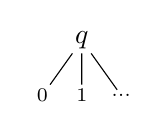
\begin{tikzpicture}[baseline=(root.base),level distance=7mm,inner ysep=0.5mm,sibling distance=5mm]
 \node (root) {$q$}
    child {node {$\scriptstyle 0$}}
    child {node {$\scriptstyle 1$}}
    child {node {$\scriptstyle \ldots$}}
;
\end{tikzpicture}$
\hspace{2cm}
$\sem{\nat \rightarrow \nat} = 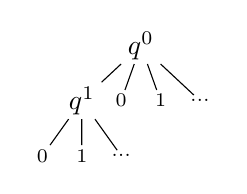
\begin{tikzpicture}[baseline=(root.base),level distance=7mm,inner ysep=0.5mm,sibling distance=5mm]
 \node (root) {$q^0$}
    child{
      node{$q^1$}
      child{node {$\scriptstyle 0$} }
      child{node {$\scriptstyle 1$} }
      child {node {$\scriptstyle \ldots$}}
    }
    child {node {$\scriptstyle 0$}}
    child {node {$\scriptstyle 1$}}
    child {node {$\scriptstyle \ldots$}}
;
\end{tikzpicture}$
\item \highlight{Play} = sequence of moves played alternatively by O and P with justification pointers.
\item \highlight{Strategy for P} = prefix-closed set of plays. $s  a  b$ in the strategy means that
P should respond $b$ when O plays $a$ in position $s$.
\item The \highlight{denotation} of a term $M$, written $\sem{M}$, is a strategy for P.
\item $\sem{ 7 : \nat} = \{ \epsilon, q, q\ 7 \}$\\
$\sem{ \pcfsucc : \nat \rightarrow \nat} = Pref( \{ q^0 q^1 n ( n+1)
\ | \ n \in \nat \} )$
\item Compositionality: $\sem{ \pcfsucc\  7} = \sem{ \pcfsucc } ; \sem{7}$
\end{itemize}
}

\frame{
\frametitle{Game semantics: composition}

\begin{itemize}
    \item Composition is done by CSP-composition + hiding:
If $\sigma : A \typear B$ and $\mu : B \typear C$ then
$$\mbox{`` }\sigma ; \mu =  (\sigma \| \mu ) \filter A,C \mbox{ ''}$$
\pause

    \item  The \highlight{fully revealed} game denotation, written $\revsem{M}$, to denote
    the set of plays obtained when hiding is never performed during composition.

    \item  The \highlight{syntactically-revealed} denotation, written $\syntrevsem{M}$, hides certain moves during composition:
in the denotation of $\revsem{x N_1\ldots N_p}$ for some variable $x$, the internal moves of $N_1$,\ldots,$N_p$ are preserved while the internal moves produced by the copy-cat projection strategy denoting $x$ are omitted.
\end{itemize}



}

\def\highlightat#1#2{\temporal<#1>{#2}{\underline{#2}}{\textcolor{blue}{#2}}}

\subsection{Computation tree}
\frame{ \frametitle{Computation tree}

We fix a simply-typed term $\Gamma \vdash M: T$.

\highlight{\it Computation tree} of $M$ is the AST of its $\eta$-long normal form.
\begin{itemize}
\item The \highlight{$\eta$-expansion} of $M:A\typear B$ is $\lambda x:A . Mx :A\typear B$.
\item The \highlight{$\eta$-long normal form} of $M$ is obtained
by hereditarily $\eta$-expanding every subterm of $M$ occurring at an operand position or as the body of a $\lambda$-abstraction.
\end{itemize}

Example:
$$h: o\typear o \vdash \lambda f^{o \typear o} .
(\lambda u^{o \typear o} . u) h : (o \typear o) \typear
o \typear o$$

\begin{columns}
\column{6cm}
Its $\eta$-long normal is
\begin{align*}
h: o \typear o &\vdash  \lambda f^{o \typear o} z^o . \\
&\qquad(\lambda u^{o \typear o} v^o . u (\lambda.v)) \\
&\qquad(\lambda y^o. h y) \\
&\qquad(\lambda.z) \\
&: (o \typear o) \typear o \typear o
\end{align*}

\column{4cm}
The computation tree is:
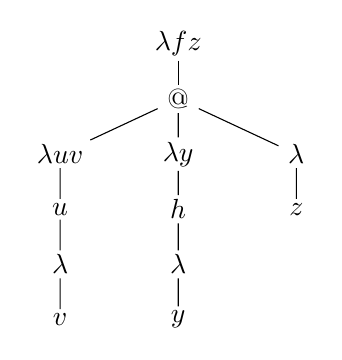
\begin{tikzpicture}[level distance=7mm,inner ysep=0.5mm]
 \node {$\lambda f z$}
    child {
        node {@}
        child {
            node {$\lambda u v$}
            child{
                node{$u$}
                child {
                    node{$\lambda$}
                    child {
                        node{$v$}
                    }
                }
            }
        }
        child {
            node {$\lambda y$}
            child{
                node {$h$}
                child{
                    node {$\lambda$}
                    child { node {$y$} }
                }
            }
        }
        child {
            node {$\lambda$}
            child{ node {$z$} }
            }
        };
\end{tikzpicture}
\end{columns}
}


\frame{
\frametitle{Justified sequence}

\begin{itemize}
\item  We define an \highlight{enabling relation} $\vdash$ on the set of nodes:
\begin{itemize}
  \item a bound variable is enabled by its binder;
  \item a free variable is enabled by the root $\theroot$;
  \item a lambda node  is enabled by its parent node;
  \item an @-node has no enabler.
\end{itemize}

\item A \highlight{justified sequence} is a sequence of nodes such that all the non @-nodes have a justification pointer respecting the relation $\vdash$.

\item  The analogy with game semantics is:
\begin{itemize}
\item $\lambda$-nodes $\equiv$ O-moves
\item @-nodes and variable-nodes $\equiv$ P-moves
\end{itemize}

We can define notions of P-view and O-view, alternation, P-visibility, O-visibility.


\item The computation will be described by a set $\travset(M)$ of justified sequences called \highlight{traversals}.
\end{itemize}
}




\frame{
\frametitle{Traversals rules}
The set $\travset(M)$ is given by induction over the rules:
%\begin{FramedTable}
%\noindent {\bf Initialization rules}
\begin{itemize}[]
\item\rulenamet{Empty} $\epsilon \in\travset(M)$
\item \rulenamet{Root} $\theroot \in \travset(M)$
%\end{itemize}
%\noindent {\bf Structural rules}
%\begin{itemize}[]
    \item \rulenamet{Lam} $t \cdot \lambda \overline{\xi} \in\travset(M) \implies t \cdot \lambda \overline{\xi} \cdot n \in\travset(M)$ where $n$
        is $\lambda \overline{\xi}$'s child and is justified by the only occurrence of
        its enabler in the P-view
    \item \rulenamet{App}  $t \cdot @ \in\travset(M) \implies$ \Pstr[0.4cm]{t \cdot (m) @  \cdot (n-m,40:0) n} $\in\travset(M)$.
%\end{itemize}
%\emph{\bf Input-variable rules}
%\begin{itemize}[]
\item \rulenamet{ContextVar} $t\cdot x\in\travset(M)$, $x\in N^{\theroot\vdash}_{\sf var}$ $\implies$
$t \cdot x \cdot n \in\travset(M)$
for any $\lambda$-node $n$ justified by some
occurrence of its parent node in $\oview{t}$.

%\item \rulenamet{ContextValue} If $t_1
%\cdot x \cdot t_2 \in\travset(M)$ with pending node $x \in
%N_{\sf var}^{\theroot\vdash}$ then so is \Pstr[0.5cm]{t_1 \cdot
%(x){x} \cdot t_2 \cdot (xv-x,38:v){v_x} } for all $v \in
%\mathcal{D}$.
%\end{itemize}
%\emph{\bf Copy-cat rules}
%\begin{itemize}[]
\item\rulenamet{Var}
\Pstr[0.2cm]{t \cdot (n){n} \cdot (lx){\lambda \overline{x}}
    \ldots (x-lx,40:i){x_i} } $\in\travset(M)$, $x_i \in
    N_{\sf var}^{@\vdash} \implies$  \Pstr[0.5cm]{ t \cdot
(n){n} \cdot (lx){\lambda \overline{x}}  \ldots (x-lx,25:i){x_i}
    \cdot (letai-n,32:i){\lambda \overline{\eta_i}}} $\in\travset(M)$.
%\item\rulenamet{Value}
%  If \Pstr{t \cdot (m){m} \cdot (n){n}  \ldots
%(vn-n,50:v){v}_{n} } $\in\travset(M)$ where $n\in N$ then
%\Pstr[0.6cm]{t \cdot (m){m} \cdot (n){n} \ldots
%(vn-n,50:v){v}_{n} \cdot (vm-m,45:v){v}_m} $\in\travset(M)$.
\end{itemize}
%\caption[Traversal rules for the simply-typed
%lambda-calculus]{Traversal rules for the simply-typed
%$\lambda$-calculus.}
%\label{tab:trav_rules}
%\end{FramedTable}

}


\frame{
\frametitle{Example of traversal}


\begin{center}
%\begin{columns}
%\column{6cm}
%\column{3.5cm}
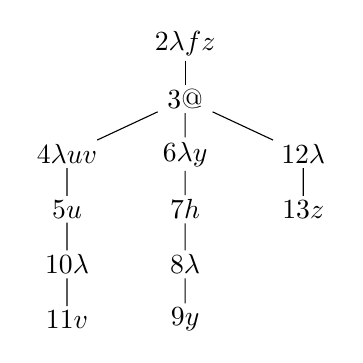
\begin{tikzpicture}[level distance=7mm,inner ysep=0.5mm]
 \node {\highlightat{2}{$\lambda f z$}}
    child {
        node {\highlightat{3}{@}}
        child {
            node {\highlightat{4}{$\lambda u v$}}
            child{
                node{\highlightat{5}{$u$}}
                child {
                    node{\highlightat{10}{$\lambda$}}
                    child {
                        node{\highlightat{11}{$v$}}
                    }
                }
            }
        }
        child {
            node {\highlightat{6}{$\lambda y$}}
            child{
                node {\highlightat{7}{$h$}}
                child{
                    node {\highlightat{8}{$\lambda$}}
                    child { node {\highlightat{9}{$y$}} }
                }
            }
        }
        child {
            node {$\highlightat{12}{\lambda}$}
            child{ node {\highlightat{13}{$z$}} }
            }
        };
\end{tikzpicture}
%\end{columns}
\end{center}

\setbox0=\hbox{$\textcolor{blue}{
\pstr{\only<2->{\nd t= (n0){\lambda f z}}
        \only<3->{\nd\cdot (n1){@}}
        \only<4->{\nd\cdot (n2-n1){\lambda u v}}
        \only<5->{\nd\cdot (n3-n2){u}}
        \only<6->{\nd\cdot (n4-n1){\lambda y}}
        \only<7->{\nd\cdot (n5-n0){h}}
        \only<8->{\nd\cdot (n6-n5){\lambda }}
        \only<9->{\nd\cdot (n7-n4){y}}
        \only<10->{\nd\cdot (n8-n3){\lambda }}
        \only<11->{\nd\cdot (n9-n2){v}}
        \only<12->{\nd\cdot (n10-n1){\lambda }}
        \only<13->{\nd\cdot (n11-n0){z}}
}}$}
\ht0 2cm\box0 % Make sure the height of box containing the traversal remains constant across the different generated slides

}

\frame{
\frametitle{Operations on traversals}
$\pstr{\nd t= (n0){\lambda f z}
        \nd\cdot (n1){@}
        \nd\cdot (n2-n1){\lambda u v}
        \nd\cdot (n3-n2){u}
        \nd\cdot (n4-n1){\lambda y}
        \nd\cdot (n5-n0){h}
        \nd\cdot (n6-n5){\lambda }
        \nd\cdot (n7-n4){y}
        \nd\cdot (n8-n3){\lambda }
        \nd\cdot (n9-n2){v}
        \nd\cdot (n10-n1){\lambda }
        \nd\cdot (n11-n0){z}
}$
\vspace*{0.4cm}
\begin{itemize}
\item The \highlight{reduction of a traversal} is obtained by keeping only
the occurrences hereditarily justified by the root:
$$\color{red}{ \Pstr[0.7cm]{t \upharpoonright r = (n0){\lambda f z}\ (n1-n0){h}\ (n2-n1){\lambda }\ (n3-n0){z} } }$$
\pause

\item  \highlight{\it @-nodes removal:}
$$\Pstr[0.5cm]{ t - @ = (n0){\lambda f z}\ (n1-n0){\lambda u v}\ (n2-n1){u}\ (n3-n0){\lambda y}\ (n4-n0){h}\ (n5-n4){\lambda }\ (n6-n3){y}\ (n7-n2){\lambda }\ (n8-n1){v}\ (n9-n0){\lambda }\ (n10-n0){z}}$$
\end{itemize}

}


\subsection{The Correspondence Theorem}
\frame{ \frametitle{The Correspondence Theorem}
\begin{block}{}
Let $M$ be a simply typed term of type $T$. There exists a partial function $\textcolor{DarkGreen}{\varphi}$
from the nodes of the \highlight{computation tree} to the
moves of the \highlight{arena} $\sem{T}$ such that
$$ \textcolor{DarkGreen}{\varphi}  : \travset(M)^{-@} \textcolor{DarkGreen}{\stackrel{\cong}{\longrightarrow}}
\syntrevsem{M} $$
$$ \textcolor{DarkGreen}{\varphi}  : \travset(M)^{\upharpoonright r}  \textcolor{DarkGreen}{\stackrel{\cong}{\longrightarrow}} \sem{M} \ .$$
\end{block}
where
\begin{itemize}
\item $\highlight{\travset(M)}$ = set of traversals of the computation tree of $M$
\item $\highlight{\travset(M)^{\upharpoonright r}} = \{ t \upharpoonright r \ | \  t \in {\travset(M)} \}$
\item $\highlight{\travset(M)^{-@}} = \{ t - @ \ | \  t \in {\travset(M)} \}$
\item $\highlight{\sem{M}}$ = game-semantic denotation of $M$
\item $\highlight{
\syntrevsem{M}}$ = syntactically-revealed denotion of $M$.
\end{itemize}

}


\frame{ \frametitle{More correspondences}
\begin{center}
\begin{tabular}{c|c}
Computation tree notions & Game-semantic equivalents \\ \hline \hline \\
computation tree & arena(s) \\ \\
traversal & uncovered play \\ \\
reduced traversal & play \\ \\
path in the computation tree & P-view of an uncovered play
\end{tabular}
\end{center}
}


\subsection{Example}
\frame{\frametitle{Example:
 $o \typear o \vdash \lambda f^{o \typear o} .
(\lambda u^{o \typear o} . u) h : (o \typear o) \typear
o \typear o$}

Left: computation tree. Right: arena.
\begin{center}
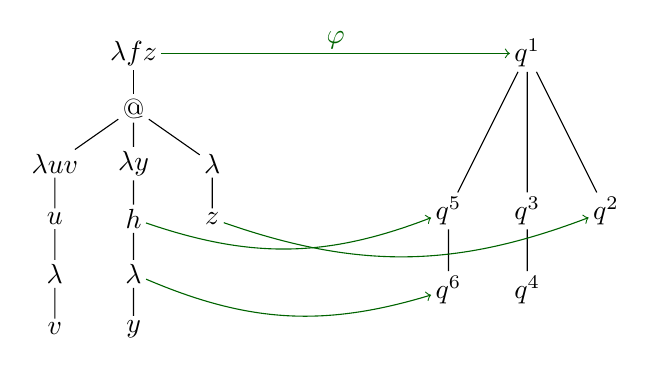
\begin{tikzpicture}[level distance=7mm,inner ysep=0.5mm,inner xsep=0.5mm,sibling distance=10mm]
%\color{blue}
\node (root) {$\lambda f z$}
    child{
      node{$@$}
          child{
            node {$\lambda u v$}
            child{
              node (u) {$u$}
              child{
                node (lmd) {$\lambda$}
                child{
                  node {$v$}
                }
              }
            }
          }
          child{
            node {$\lambda y$}
            child{
                node (h) {$h$}
                child{
                  node (h1) {$\lambda$}
                  child{
                    node {$y$}
                  }
                }
            }
          }
          child{
            node {$\lambda$}
            child{
              node (z) {$z$}
            }
          }
      }
;
%\color{red}
\draw +(5,0) node (q1) {$q^1$}
    [level distance=20mm]
      child{
        node (q5) {$q^5$}
        [level distance=10mm]
        child{ node (q6) {$q^6$} }
      }
      child{
        node (q3) {$q^3$}
        [level distance=10mm]
        child{ node (q4) {$q^4$} }
      }
      child{ node (q2) {$q^2$} }
;
\color{DarkGreen}
\draw[->] (root) -- node[above] {$\varphi$} (q1);
\draw[->] (h) to [bend right=20]  (q5);
\draw[->] (h1) to [bend right=20]  (q6);
\draw[->] (z) to [bend right=20]  (q2);
\end{tikzpicture}
\end{center}
\begin{itemize}
\item $\pstr{\nd t= (n0){\lambda f z}
        \nd\cdot (n1){@}
        \nd\cdot (n2-n1,35){\lambda u v}
        \nd\cdot (n3-n2,35){u}
        \nd\cdot (n4-n1,35){\lambda y}
        \nd\cdot (n5-n0,35){h}
        \nd\cdot (n6-n5,35){\lambda }
        \nd\cdot (n7-n4,35){y}
        \nd\cdot (n8-n3,35){\lambda }
        \nd\cdot (n9-n2,35){v}
        \nd\cdot (n10-n1,35){\lambda }
        \nd\cdot (n11-n0,35){z}
}$

\item $\Pstr{\pview{t} = (q1){\lambda f z} \cdot (n2){@}
\cdot (n9-n2,35){\lambda}
\cdot (q2-q1,35){z}}$

\item
$
\textcolor{DarkGreen}{
\varphi (} %\textcolor{blue}
{t \upharpoonright r}
\textcolor{DarkGreen}{)} = \textcolor{DarkGreen}{\varphi (}
\textcolor{blue}{
\Pstr[70mm]{ (q1){\lambda f z}
            \cdot (q3-q1){h}
            \cdot (q4-q3){\lambda}
            \cdot (q2-q1){z} }
}
\textcolor{DarkGreen}{)} = %\textcolor{red}
{
\Pstr[70mm]{
    (q1){q}^1\
    (q5-q1){q}^5\
    (q6-q3){q}^6\
    (q2-q1){q}^2
}}
\in %\textcolor{red}
{\sem{M}}.
$

\end{itemize}
}



\begingroup
\newcommand\sigcol[1]{{\color{blue} #1}}
\newcommand\mucol[1]{{\color{red} #1}}
\newcommand\mynodeex[2]{\node[name=#1]{$#2$};}

\subsection{Composition}
\begin{frame}[fragile]
\frametitle{Composition}

Take $\sigcol{\sigma} = \sem{ \vdash \sigcol{\lambda x^o v^o .x} : o\typear (o,o)}$
 and  $\mucol{\mu} = \sem{ \vdash \mucol{\lambda y^{(o,o)} \varphi^{((o,o),o)}. \varphi (\lambda u^o . y~u)} : (o,o) \typear (((o,o),o),o)}$.

We then have $\sigcol{\sigma} \fatcompos \mucol{\mu} = \sem{ \lambda x \varphi. \varphi (\lambda u . x) : o \typear (((o,o),o),o)}$.
\bigskip

\begin{tikzpicture}
  [every node/.style={anchor=base}]
  \matrix [matrix of nodes]
  {
    o & $\stackrel{\sigcol{\sigma}}\longrightarrow$ & (o,& o) & $\stackrel{\mucol{\mu}}\longrightarrow$ &  (((o,&o),&o), & o) \\
&&&&&&&&\mynodeex{n0}{\lambda x \varphi \omove  \mucol {\lambda y \varphi}}\\
&&&&&&&\mynodeex{n1}{\varphi  \pmove \mucol \varphi}\\
&&&&&&\mynodeex{n2}{\lambda u \omove  \mucol {\lambda u}} \\
&&&  \mynodeex{n3}{\sigcol {\lambda x v} \opmove \mucol y} \\
\mynodeex{n4}{x \pmove \sigcol x}\\
  };
\draw[->] (n4) .. controls +(60:1cm) and +(-1,0) .. (n0.west);
\draw[->] (n2) .. controls +(60:0.2cm) and +(-0.4cm,0) .. (n1.west);
\draw[->] (n1) .. controls +(60:0.2cm) and +(-0.4cm,0) .. (n0.west);
\draw[->] (n3) .. controls +(30:1cm) and +(-1,0) .. (n0.west);
\draw[->] (n4) .. controls +(30:1cm) and +(-1,0) .. (n3.west);
\end{tikzpicture}
\end{frame}
\endgroup


\subsection{Demo}
\frame{\frametitle{Tool demo}
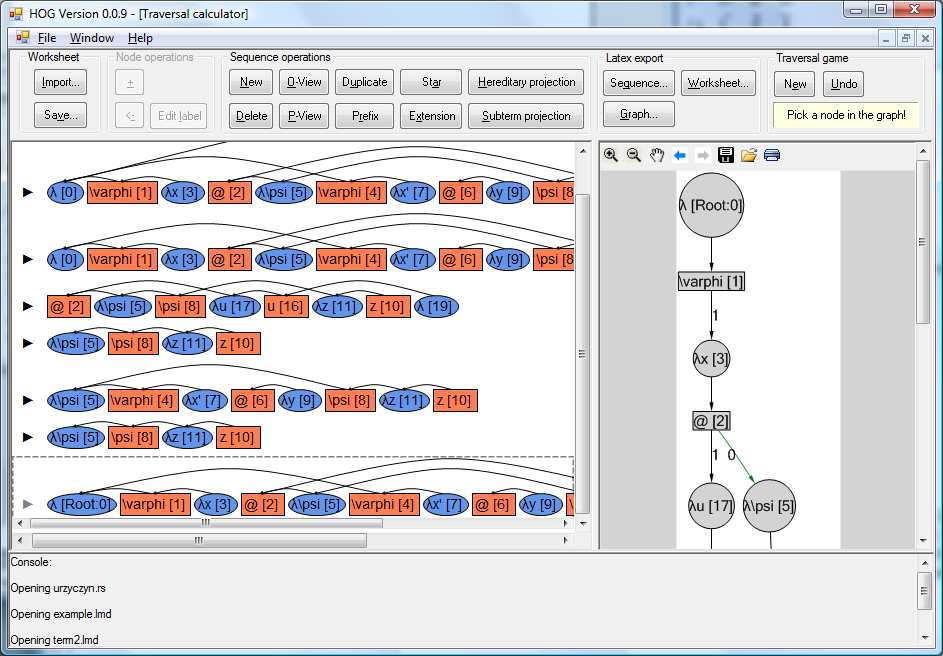
\includegraphics[width=11cm]{sshot.jpg}

}




%%%%%%%%%%%%%%%%%%%%%%%%%%%%%%%%%%%%%%%%%%%%%%%%%

\section{Applications}


\subsection{Higher-order grammars}
\frame{\frametitle{Higher-order grammars}
\emph{Notation for types:} $A_1 \rightarrow (A_2 \rightarrow (\ldots (A_n \rightarrow o)) \ldots )$
is written $(A_1,A_2,\ldots, A_n,o)$.

\begin{itemize}

\item Higher-order grammars used as generators of word languages, trees or graphs  are called \highlight{recursion schemes} (Maslov, 1974).

\item A \highlight{higher-order grammar} is formally given by a tuple
$\langle \Sigma, \mathcal{N}, \mathcal{R}, \mathcal{S} \rangle$
(terminals, non-terminals, rewritting rules, starting symbol)

\item Example of a tree-generating order-2 recursion scheme:
\begin{columns}
      \column{.3\textwidth}
$\begin{array}{rll}
  S & \rightarrow & H \, a\\
  H \, z^o & \rightarrow & F \, (g \,
  z)\\
  F \, \phi^{(o, o)} & \rightarrow & \phi \, (\phi \, (F \, h))\\
\end{array}$
      \column{.3\textwidth}
\begin{tikzpicture}[baseline=(root.base),level distance=5mm,inner ysep=0.5mm,sibling distance=10mm]
 \node (root) {$g$}
    child {node {$a$}}
    child {node {$g$}
        child { node{$a$} }
        child { node{$h$}
                child { node{$h$}
                        child { node{$\vdots$} }
                }
        }
    } ;
\end{tikzpicture}
\end{columns}
Non-terminals: $S :o$, $H:(o,o)$ and $F:((o,o),o)$. Terminals: $a:o$ and $g,h:(o,o)$.
\end{itemize}
}

\frame{
\frametitle{Tree generating HO-PDA}
Higher-order pushdown automata (HOPDA)
generalize PDA to nested stacks. An 1-PDA is a standard PDA. An order $n$-HOPDA manipulates a stack with $n$ levels of nesting.

The transitions are of the following kinds:
\begin{itemize}
    \item $push_1 a$: push the element $a$ on the top level $1$-stack;
    \item $pop_1$: pop the top element of the top level $1$-stack;
    \item $push_n$, $n>1$: duplicate the top level $n-1$-stack;
    \item $pop_n$, $n>1$: delete the top level $n-1$-stack.
\end{itemize}
Additionally, since we use HOPDA to generate a tree, we have:
\begin{itemize}
  \item $emit_f (q_1, \ldots, q_k)$, for each node-constructor $f:o^k\typear \in \Sigma$.
\end{itemize}

\begin{theorem}
For generating word or tree languages, order-$n$ pushdown automata
are equivalent to order-$n$ \highlight{safe} grammars [Damm82,KNU02].
\end{theorem}
}

\frame{
\frametitle{Collapsible PDA}

What is the automaton equivalent of unrestricted grammars?
\pause

\begin{itemize}
\item Answer: Collapsible Pushdown Automaton CPDA [Hague,Murawski,Ong,Serre, LICS08]:
\begin{itemize}
    \item it is an extension of HO-PDA where each symbol in the stack can have a pointer to a sub-stack occurring underneath it;
    \item it can ``collapse'' the stack by following the pointer associated to the top element.
\end{itemize}

\item There is a transformation from HORS to CPDA and reciprocally.

\item The first transformation is based on the traversal framework:
\begin{enumerate}[1.]
  \item compute the computation graph of the HORS by taking the $\eta$-long nf of each grammar rule;
  \item construct a CPDA ``simulating'' the HORS by calculating the traversal of its computation graph.
\end{enumerate}
\pause
\item Tool demo...
\end{itemize}

}

\subsection{Other applications}
\frame{\frametitle{Other applications, related works}

\begin{itemize}
\item \highlight{Verification:}  Knapik {\it et.\ al.} (2002) showed that \highlight{MSO model checking} for trees generated by HORS
 of any order and verifying the \highlight{safety restriction} (a syntactic restriction that constrains the occurrences of variables according to their orders) is decidable.

    Using the notions of computation tree/traversal Ong was able to show (LICS06) that this result still holds in the unrestricted case.
%\item Ong introduced computation trees in LICS2006 to prove decidability of MSO theory on infinite trees
%generated by higher-order grammars.

\pause

\item Studying the effect of syntactic restrictions on the game semantics model.
 \eg\ One can show that \highlight{pointers are uniquely recoverable} in the game denotation of terms satisfying the safety restriction.
\pause

\end{itemize}

\highlight{Related works:}

\begin{itemize}
\item Stirling recently proved decidability of higher-order pattern matching with a game-semantic approach
 relying on equivalent notions of computation tree and traversal.
\end{itemize}
}



%%%%%%%%%%%%%%%%%%%%%%%%%%%%%%%%%%%%%%%%%%%%%%%%%
%\subsection{Simply Typed \texorpdfstring{$\lambda$}{Lambda}-Calculus}
%\frame{\frametitle{Simply Typed $\lambda$-Calculus}
%\begin{itemize}
%\item \highlight{Simple types} $A := o\ |\ A \rightarrow A$.
%%We write $(A_1,\ldots, A_n)$ for $A_1\rightarrow \ldots \rightarrow A_n$.
%
%\item The \highlight{order} of a type is given by $\textsf{order}(o) = 0$,
%$\textsf{order}(A \rightarrow B) = \max(\textsf{order}(A) + 1, \textsf{order}(B))$.
%
%
%\end{itemize}
%}
%



\section{Future Works}
\frame{ \frametitle{Future Works}

%\highlight{Future works:}
\begin{itemize}
\item Implement other transformations: from CPDA to HORS and from safe HORS to PDA.
\item Implement the MSO decision procedure.
\item Application to implicit complexity: can we obtain space-complexity characterizations by analyzing the length of the traversals? (See Kazushige Terui's work.)
\end{itemize}


}

\begin{frame} \frametitle<presentation>{Bibliography}

  \begin{thebibliography}{10}
  \beamertemplatearticlebibitems
    \bibitem{abramsky:game-semantics-tutorial}
    Samson Abramsky and Guy McCusker.
    \newblock Game semantics, Lecture notes.
    \newblock In {\em Proceedings of the 1997 Marktoberdorf Summer School}. Springer-Verlag, 1998.

%    \bibitem{safety-mirlong2004}
%    Klaus Aehlig, Jolie~G. de~Miranda, and C.-H.~Luke Ong.
%    \newblock Safety is not a restriction at level 2 for string languages.
%    \newblock Technical report. University of Oxford, 2004.

    \bibitem{hague-sto07}
    M.~Hague, A.S.~Murawski, C.-H.~L. Ong and O.~Serre.
    \newblock Collapsible pushdown automata and recursive schemes.
    \newblock To appear, LICS2008.

    \bibitem{OngLics2006}
    C.-H.~Luke Ong.
    \newblock On model-checking trees generated by higher-order recursion schemes.
    \newblock In {\em Proceedings of LICS.} Computer Society Press, 2006.

    \bibitem{DBLP:conf/icalp/Stirling06}
    Colin Stirling
    \newblock A Game-Theoretic Approach to Deciding Higher-Order Matching.
    \newblock In {\em Proceedings of ICALP.} Springer, 2006.

  \end{thebibliography}
\end{frame}




\note{
\begin{itemize}
\item nPDA = finite state machines + order n stack
\item For words: 1PDA recognizes context-free language.
        and 0PDA = recognizes regular language.
\item MSO is very expressive: more than the modal mu-calculus (into which LTL CTL CTL* can be embedded.
But over trees, MSO and modal mu-calculus are equi-expressive.)
\item [Caucal02] Graphs generated by safe grammars have a decidable MSO theory.
\item [HMOS06] Caucal's result does not extend to unsafe grammars.
However deciding $\mu$-calculus theories is $n$-EXPTIME complete.
\end{itemize}
}


\end{document}

\def\toolname{HOG}

\pstrSetArrowColor{black}

\title{\texorpdfstring{A Concrete Presentation of Game Semantics}{A Concrete Presentation of Game Semantics}}

\author[W. Blum, C.-H. L. Ong]{\texorpdfstring{\\ William Blum\\ \ \\
 Joint work with C.-H. Luke Ong}{William Blum}}


\institute[Oxford University -- Edinburgh University]{School of Informatics, University of Edinburgh -- Oxford University Computing Laboratory}

\date{\small \color{red}{Galop 2008, 5 April 2008}}


\begin{document}

\frame{\titlepage}

\frame{\frametitle{Overview}
\begin{itemize}
  \item
Game-semantic model are \highlight{abstract} \ie independent of the syntax of the denotated term. We give here a \highlight{concrete} \ie syntactic representation of game semantics where:
\begin{itemize}
\item The arena game is incarnated by some abstract syntax tree of the term.
\item Plays become traversals over this tree.
\end{itemize}


\item A ``Correspondence Theorem'' establishes the relationship between the game-semantic and traversal models.

\item We developed the tool \toolname\ to illustrate this correspondence.

\item Example of application:
computing infinite trees generated by \emph{higher-order recursion scheme}.
\end{itemize}



%We briefly present a new representation theory for game semantics which is very concrete: instead of playing in an arena game in which P plays the innocent strategy given by a term, the same game is played out over (a souped up version of) the abstract syntax tree of the term itself. The plays that are thus traced out are called \highlight{traversals}. More abstractly, traversals are the justified sequences that are obtained by performing parallel-composition \emph{less} the hiding. After stating and explaining a number of Path-Traversal Correspondence Theorems, we present a tool for game semantics based on the new representation.

}


%\section<presentation>*{Outline}
\begin{frame}
  \frametitle{Outline}
  \tableofcontents
\end{frame}

\AtBeginSection[] {
   \begin{frame}
     \frametitle{Outline}
     \tableofcontents[currentpart,currentsection]
   \end{frame}
 }


%%%%%%%%%%%%%%%%%%%%%%%%%%%%%%%%%%%%%%%%%%%%%%%%%
\section{The correspondence}

\subsection{Game semantics}

%%% The Correspondence in one slide
%\frame{ \frametitle{Correspondence Theorem}
%Let $\vdash M:T$ be a pure simply typed term.
%
%\begin{itemize}
%\item \highlight{Game-semantics} provides a model of $\lambda$-calculus.
%$M$ is denoted by a strategy $\sem{M}$ on a 2-player game induced by $T$.
%\item A \highlight{strategy} is represented by a set of sequences of moves together with \highlight{links}: each move points
%to a preceding move.
%\pause
%\item \textcolor{DarkGreen}{Computation tree} = canonical tree representation of a term.
%\item \textcolor{DarkGreen}{Traversals $\travset(M)$ } = sequences of nodes with links respecting some formation rules.
%\end{itemize}
%\pause
%
%\begin{block}{The Correspondence Theorem}
%The game semantics of a term can be represented on the computation
%tree:
%$$ \textcolor{DarkGreen}{\travset(M)} \cong \textcolor{blue}{\intersem{M}} $$
%$$ \textcolor{DarkGreen}{Reduction(\travset(M))} \cong \textcolor{blue}{\sem{M}}$$
%where $\textcolor{blue}{\intersem{M}}$ is the revealed game-semantic denotion (i.e. internal moves are uncovered).
%\end{block}
%}

\frame{\frametitle{Game semantics}
 Model of programming languages based on games (Abramsky et al.; Hyland and Ong; Nickau)
\begin{itemize}
\item 2 players: \highlight{O}pponnent (system) and \highlight{P}roponent (program)
\item The term type induces an \highlight{arena} defining the possible moves
$\sem{\nat} = 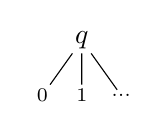
\begin{tikzpicture}[baseline=(root.base),level distance=7mm,inner ysep=0.5mm,sibling distance=5mm]
 \node (root) {$q$}
    child {node {$\scriptstyle 0$}}
    child {node {$\scriptstyle 1$}}
    child {node {$\scriptstyle \ldots$}}
;
\end{tikzpicture}$
\hspace{2cm}
$\sem{\nat \rightarrow \nat} = 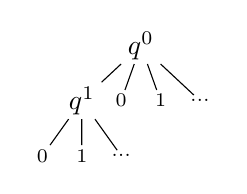
\begin{tikzpicture}[baseline=(root.base),level distance=7mm,inner ysep=0.5mm,sibling distance=5mm]
 \node (root) {$q^0$}
    child{
      node{$q^1$}
      child{node {$\scriptstyle 0$} }
      child{node {$\scriptstyle 1$} }
      child {node {$\scriptstyle \ldots$}}
    }
    child {node {$\scriptstyle 0$}}
    child {node {$\scriptstyle 1$}}
    child {node {$\scriptstyle \ldots$}}
;
\end{tikzpicture}$
\item \highlight{Play} = sequence of moves played alternatively by O and P with justification pointers.
\item \highlight{Strategy for P} = prefix-closed set of plays. $s  a  b$ in the strategy means that
P should respond $b$ when O plays $a$ in position $s$.
\item The \highlight{denotation} of a term $M$, written $\sem{M}$, is a strategy for P.
\item $\sem{ 7 : \nat} = \{ \epsilon, q, q\ 7 \}$\\
$\sem{ \pcfsucc : \nat \rightarrow \nat} = Pref( \{ q^0 q^1 n ( n+1)
\ | \ n \in \nat \} )$
\item Compositionality: $\sem{ \pcfsucc\  7} = \sem{ \pcfsucc } ; \sem{7}$
\end{itemize}
}

\frame{
\frametitle{Game semantics: composition}

\begin{itemize}
    \item Composition is done by CSP-composition + hiding:
If $\sigma : A \typear B$ and $\mu : B \typear C$ then
$$\mbox{`` }\sigma ; \mu =  (\sigma \| \mu ) \filter A,C \mbox{ ''}$$
\pause

    \item  The \highlight{fully revealed} game denotation, written $\revsem{M}$, to denote
    the set of plays obtained when hiding is never performed during composition.

    \item  The \highlight{syntactically-revealed} denotation, written $\syntrevsem{M}$, hides certain moves during composition:
in the denotation of $\revsem{x N_1\ldots N_p}$ for some variable $x$, the internal moves of $N_1$,\ldots,$N_p$ are preserved while the internal moves produced by the copy-cat projection strategy denoting $x$ are omitted.
\end{itemize}



}

\def\highlightat#1#2{\temporal<#1>{#2}{\underline{#2}}{\textcolor{blue}{#2}}}

\subsection{Computation tree}
\frame{ \frametitle{Computation tree}

We fix a simply-typed term $\Gamma \vdash M: T$.

\highlight{\it Computation tree} of $M$ is the AST of its $\eta$-long normal form.
\begin{itemize}
\item The \highlight{$\eta$-expansion} of $M:A\typear B$ is $\lambda x:A . Mx :A\typear B$.
\item The \highlight{$\eta$-long normal form} of $M$ is obtained
by hereditarily $\eta$-expanding every subterm of $M$ occurring at an operand position or as the body of a $\lambda$-abstraction.
\end{itemize}

Example:
$$h: o\typear o \vdash \lambda f^{o \typear o} .
(\lambda u^{o \typear o} . u) h : (o \typear o) \typear
o \typear o$$

\begin{columns}
\column{6cm}
Its $\eta$-long normal is
\begin{align*}
h: o \typear o &\vdash  \lambda f^{o \typear o} z^o . \\
&\qquad(\lambda u^{o \typear o} v^o . u (\lambda.v)) \\
&\qquad(\lambda y^o. h y) \\
&\qquad(\lambda.z) \\
&: (o \typear o) \typear o \typear o
\end{align*}

\column{4cm}
The computation tree is:
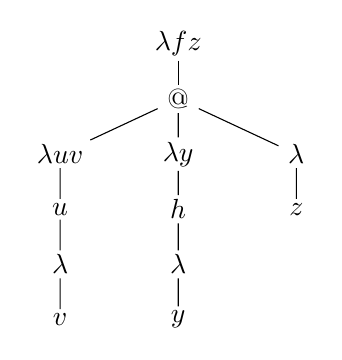
\begin{tikzpicture}[level distance=7mm,inner ysep=0.5mm]
 \node {$\lambda f z$}
    child {
        node {@}
        child {
            node {$\lambda u v$}
            child{
                node{$u$}
                child {
                    node{$\lambda$}
                    child {
                        node{$v$}
                    }
                }
            }
        }
        child {
            node {$\lambda y$}
            child{
                node {$h$}
                child{
                    node {$\lambda$}
                    child { node {$y$} }
                }
            }
        }
        child {
            node {$\lambda$}
            child{ node {$z$} }
            }
        };
\end{tikzpicture}
\end{columns}
}


\frame{
\frametitle{Justified sequence}

\begin{itemize}
\item  We define an \highlight{enabling relation} $\vdash$ on the set of nodes:
\begin{itemize}
  \item a bound variable is enabled by its binder;
  \item a free variable is enabled by the root $\theroot$;
  \item a lambda node  is enabled by its parent node;
  \item an @-node has no enabler.
\end{itemize}

\item A \highlight{justified sequence} is a sequence of nodes such that all the non @-nodes have a justification pointer respecting the relation $\vdash$.

\item  The analogy with game semantics is:
\begin{itemize}
\item $\lambda$-nodes $\equiv$ O-moves
\item @-nodes and variable-nodes $\equiv$ P-moves
\end{itemize}

We can define notions of P-view and O-view, alternation, P-visibility, O-visibility.


\item The computation will be described by a set $\travset(M)$ of justified sequences called \highlight{traversals}.
\end{itemize}
}




\frame{
\frametitle{Traversals rules}
The set $\travset(M)$ is given by induction over the rules:
%\begin{FramedTable}
%\noindent {\bf Initialization rules}
\begin{itemize}[]
\item\rulenamet{Empty} $\epsilon \in\travset(M)$
\item \rulenamet{Root} $\theroot \in \travset(M)$
%\end{itemize}
%\noindent {\bf Structural rules}
%\begin{itemize}[]
    \item \rulenamet{Lam} $t \cdot \lambda \overline{\xi} \in\travset(M) \implies t \cdot \lambda \overline{\xi} \cdot n \in\travset(M)$ where $n$
        is $\lambda \overline{\xi}$'s child and is justified by the only occurrence of
        its enabler in the P-view
    \item \rulenamet{App}  $t \cdot @ \in\travset(M) \implies$ \Pstr[0.4cm]{t \cdot (m) @  \cdot (n-m,40:0) n} $\in\travset(M)$.
%\end{itemize}
%\emph{\bf Input-variable rules}
%\begin{itemize}[]
\item \rulenamet{ContextVar} $t\cdot x\in\travset(M)$, $x\in N^{\theroot\vdash}_{\sf var}$ $\implies$
$t \cdot x \cdot n \in\travset(M)$
for any $\lambda$-node $n$ justified by some
occurrence of its parent node in $\oview{t}$.

%\item \rulenamet{ContextValue} If $t_1
%\cdot x \cdot t_2 \in\travset(M)$ with pending node $x \in
%N_{\sf var}^{\theroot\vdash}$ then so is \Pstr[0.5cm]{t_1 \cdot
%(x){x} \cdot t_2 \cdot (xv-x,38:v){v_x} } for all $v \in
%\mathcal{D}$.
%\end{itemize}
%\emph{\bf Copy-cat rules}
%\begin{itemize}[]
\item\rulenamet{Var}
\Pstr[0.2cm]{t \cdot (n){n} \cdot (lx){\lambda \overline{x}}
    \ldots (x-lx,40:i){x_i} } $\in\travset(M)$, $x_i \in
    N_{\sf var}^{@\vdash} \implies$  \Pstr[0.5cm]{ t \cdot
(n){n} \cdot (lx){\lambda \overline{x}}  \ldots (x-lx,25:i){x_i}
    \cdot (letai-n,32:i){\lambda \overline{\eta_i}}} $\in\travset(M)$.
%\item\rulenamet{Value}
%  If \Pstr{t \cdot (m){m} \cdot (n){n}  \ldots
%(vn-n,50:v){v}_{n} } $\in\travset(M)$ where $n\in N$ then
%\Pstr[0.6cm]{t \cdot (m){m} \cdot (n){n} \ldots
%(vn-n,50:v){v}_{n} \cdot (vm-m,45:v){v}_m} $\in\travset(M)$.
\end{itemize}
%\caption[Traversal rules for the simply-typed
%lambda-calculus]{Traversal rules for the simply-typed
%$\lambda$-calculus.}
%\label{tab:trav_rules}
%\end{FramedTable}

}


\frame{
\frametitle{Example of traversal}


\begin{center}
%\begin{columns}
%\column{6cm}
%\column{3.5cm}
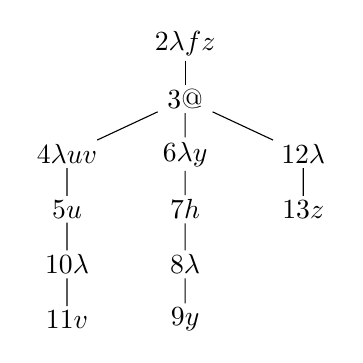
\begin{tikzpicture}[level distance=7mm,inner ysep=0.5mm]
 \node {\highlightat{2}{$\lambda f z$}}
    child {
        node {\highlightat{3}{@}}
        child {
            node {\highlightat{4}{$\lambda u v$}}
            child{
                node{\highlightat{5}{$u$}}
                child {
                    node{\highlightat{10}{$\lambda$}}
                    child {
                        node{\highlightat{11}{$v$}}
                    }
                }
            }
        }
        child {
            node {\highlightat{6}{$\lambda y$}}
            child{
                node {\highlightat{7}{$h$}}
                child{
                    node {\highlightat{8}{$\lambda$}}
                    child { node {\highlightat{9}{$y$}} }
                }
            }
        }
        child {
            node {$\highlightat{12}{\lambda}$}
            child{ node {\highlightat{13}{$z$}} }
            }
        };
\end{tikzpicture}
%\end{columns}
\end{center}

\setbox0=\hbox{$\textcolor{blue}{
\pstr{\only<2->{\nd t= (n0){\lambda f z}}
        \only<3->{\nd\cdot (n1){@}}
        \only<4->{\nd\cdot (n2-n1){\lambda u v}}
        \only<5->{\nd\cdot (n3-n2){u}}
        \only<6->{\nd\cdot (n4-n1){\lambda y}}
        \only<7->{\nd\cdot (n5-n0){h}}
        \only<8->{\nd\cdot (n6-n5){\lambda }}
        \only<9->{\nd\cdot (n7-n4){y}}
        \only<10->{\nd\cdot (n8-n3){\lambda }}
        \only<11->{\nd\cdot (n9-n2){v}}
        \only<12->{\nd\cdot (n10-n1){\lambda }}
        \only<13->{\nd\cdot (n11-n0){z}}
}}$}
\ht0 2cm\box0 % Make sure the height of box containing the traversal remains constant across the different generated slides

}

\frame{
\frametitle{Operations on traversals}
$\pstr{\nd t= (n0){\lambda f z}
        \nd\cdot (n1){@}
        \nd\cdot (n2-n1){\lambda u v}
        \nd\cdot (n3-n2){u}
        \nd\cdot (n4-n1){\lambda y}
        \nd\cdot (n5-n0){h}
        \nd\cdot (n6-n5){\lambda }
        \nd\cdot (n7-n4){y}
        \nd\cdot (n8-n3){\lambda }
        \nd\cdot (n9-n2){v}
        \nd\cdot (n10-n1){\lambda }
        \nd\cdot (n11-n0){z}
}$
\vspace*{0.4cm}
\begin{itemize}
\item The \highlight{reduction of a traversal} is obtained by keeping only
the occurrences hereditarily justified by the root:
$$\color{red}{ \Pstr[0.7cm]{t \upharpoonright r = (n0){\lambda f z}\ (n1-n0){h}\ (n2-n1){\lambda }\ (n3-n0){z} } }$$
\pause

\item  \highlight{\it @-nodes removal:}
$$\Pstr[0.5cm]{ t - @ = (n0){\lambda f z}\ (n1-n0){\lambda u v}\ (n2-n1){u}\ (n3-n0){\lambda y}\ (n4-n0){h}\ (n5-n4){\lambda }\ (n6-n3){y}\ (n7-n2){\lambda }\ (n8-n1){v}\ (n9-n0){\lambda }\ (n10-n0){z}}$$
\end{itemize}

}


\subsection{The Correspondence Theorem}
\frame{ \frametitle{The Correspondence Theorem}
\begin{block}{}
Let $M$ be a simply typed term of type $T$. There exists a partial function $\textcolor{DarkGreen}{\varphi}$
from the nodes of the \highlight{computation tree} to the
moves of the \highlight{arena} $\sem{T}$ such that
$$ \textcolor{DarkGreen}{\varphi}  : \travset(M)^{-@} \textcolor{DarkGreen}{\stackrel{\cong}{\longrightarrow}}
\syntrevsem{M} $$
$$ \textcolor{DarkGreen}{\varphi}  : \travset(M)^{\upharpoonright r}  \textcolor{DarkGreen}{\stackrel{\cong}{\longrightarrow}} \sem{M} \ .$$
\end{block}
where
\begin{itemize}
\item $\highlight{\travset(M)}$ = set of traversals of the computation tree of $M$
\item $\highlight{\travset(M)^{\upharpoonright r}} = \{ t \upharpoonright r \ | \  t \in {\travset(M)} \}$
\item $\highlight{\travset(M)^{-@}} = \{ t - @ \ | \  t \in {\travset(M)} \}$
\item $\highlight{\sem{M}}$ = game-semantic denotation of $M$
\item $\highlight{
\syntrevsem{M}}$ = syntactically-revealed denotion of $M$.
\end{itemize}

}


\frame{ \frametitle{More correspondences}
\begin{center}
\begin{tabular}{c|c}
Computation tree notions & Game-semantic equivalents \\ \hline \hline \\
computation tree & arena(s) \\ \\
traversal & uncovered play \\ \\
reduced traversal & play \\ \\
path in the computation tree & P-view of an uncovered play
\end{tabular}
\end{center}
}


\subsection{Example}
\frame{\frametitle{Example:
 $o \typear o \vdash \lambda f^{o \typear o} .
(\lambda u^{o \typear o} . u) h : (o \typear o) \typear
o \typear o$}

Left: computation tree. Right: arena.
\begin{center}
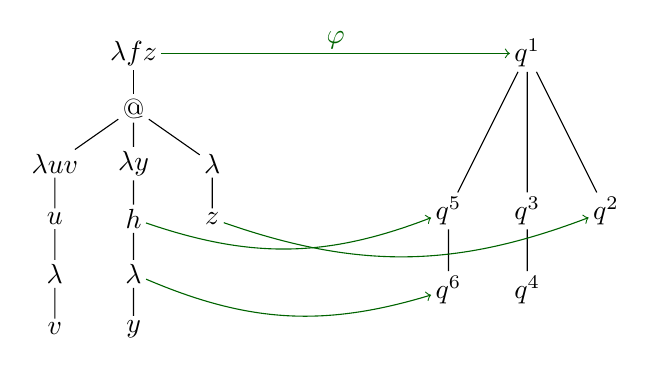
\begin{tikzpicture}[level distance=7mm,inner ysep=0.5mm,inner xsep=0.5mm,sibling distance=10mm]
%\color{blue}
\node (root) {$\lambda f z$}
    child{
      node{$@$}
          child{
            node {$\lambda u v$}
            child{
              node (u) {$u$}
              child{
                node (lmd) {$\lambda$}
                child{
                  node {$v$}
                }
              }
            }
          }
          child{
            node {$\lambda y$}
            child{
                node (h) {$h$}
                child{
                  node (h1) {$\lambda$}
                  child{
                    node {$y$}
                  }
                }
            }
          }
          child{
            node {$\lambda$}
            child{
              node (z) {$z$}
            }
          }
      }
;
%\color{red}
\draw +(5,0) node (q1) {$q^1$}
    [level distance=20mm]
      child{
        node (q5) {$q^5$}
        [level distance=10mm]
        child{ node (q6) {$q^6$} }
      }
      child{
        node (q3) {$q^3$}
        [level distance=10mm]
        child{ node (q4) {$q^4$} }
      }
      child{ node (q2) {$q^2$} }
;
\color{DarkGreen}
\draw[->] (root) -- node[above] {$\varphi$} (q1);
\draw[->] (h) to [bend right=20]  (q5);
\draw[->] (h1) to [bend right=20]  (q6);
\draw[->] (z) to [bend right=20]  (q2);
\end{tikzpicture}
\end{center}
\begin{itemize}
\item $\pstr{\nd t= (n0){\lambda f z}
        \nd\cdot (n1){@}
        \nd\cdot (n2-n1,35){\lambda u v}
        \nd\cdot (n3-n2,35){u}
        \nd\cdot (n4-n1,35){\lambda y}
        \nd\cdot (n5-n0,35){h}
        \nd\cdot (n6-n5,35){\lambda }
        \nd\cdot (n7-n4,35){y}
        \nd\cdot (n8-n3,35){\lambda }
        \nd\cdot (n9-n2,35){v}
        \nd\cdot (n10-n1,35){\lambda }
        \nd\cdot (n11-n0,35){z}
}$

\item $\Pstr{\pview{t} = (q1){\lambda f z} \cdot (n2){@}
\cdot (n9-n2,35){\lambda}
\cdot (q2-q1,35){z}}$

\item
$
\textcolor{DarkGreen}{
\varphi (} %\textcolor{blue}
{t \upharpoonright r}
\textcolor{DarkGreen}{)} = \textcolor{DarkGreen}{\varphi (}
\textcolor{blue}{
\Pstr[70mm]{ (q1){\lambda f z}
            \cdot (q3-q1){h}
            \cdot (q4-q3){\lambda}
            \cdot (q2-q1){z} }
}
\textcolor{DarkGreen}{)} = %\textcolor{red}
{
\Pstr[70mm]{
    (q1){q}^1\
    (q5-q1){q}^5\
    (q6-q3){q}^6\
    (q2-q1){q}^2
}}
\in %\textcolor{red}
{\sem{M}}.
$

\end{itemize}
}



\begingroup
\newcommand\sigcol[1]{{\color{blue} #1}}
\newcommand\mucol[1]{{\color{red} #1}}
\newcommand\mynodeex[2]{\node[name=#1]{$#2$};}

\subsection{Composition}
\begin{frame}[fragile]
\frametitle{Composition}

Take $\sigcol{\sigma} = \sem{ \vdash \sigcol{\lambda x^o v^o .x} : o\typear (o,o)}$
 and  $\mucol{\mu} = \sem{ \vdash \mucol{\lambda y^{(o,o)} \varphi^{((o,o),o)}. \varphi (\lambda u^o . y~u)} : (o,o) \typear (((o,o),o),o)}$.

We then have $\sigcol{\sigma} \fatcompos \mucol{\mu} = \sem{ \lambda x \varphi. \varphi (\lambda u . x) : o \typear (((o,o),o),o)}$.
\bigskip

\begin{tikzpicture}
  [every node/.style={anchor=base}]
  \matrix [matrix of nodes]
  {
    o & $\stackrel{\sigcol{\sigma}}\longrightarrow$ & (o,& o) & $\stackrel{\mucol{\mu}}\longrightarrow$ &  (((o,&o),&o), & o) \\
&&&&&&&&\mynodeex{n0}{\lambda x \varphi \omove  \mucol {\lambda y \varphi}}\\
&&&&&&&\mynodeex{n1}{\varphi  \pmove \mucol \varphi}\\
&&&&&&\mynodeex{n2}{\lambda u \omove  \mucol {\lambda u}} \\
&&&  \mynodeex{n3}{\sigcol {\lambda x v} \opmove \mucol y} \\
\mynodeex{n4}{x \pmove \sigcol x}\\
  };
\draw[->] (n4) .. controls +(60:1cm) and +(-1,0) .. (n0.west);
\draw[->] (n2) .. controls +(60:0.2cm) and +(-0.4cm,0) .. (n1.west);
\draw[->] (n1) .. controls +(60:0.2cm) and +(-0.4cm,0) .. (n0.west);
\draw[->] (n3) .. controls +(30:1cm) and +(-1,0) .. (n0.west);
\draw[->] (n4) .. controls +(30:1cm) and +(-1,0) .. (n3.west);
\end{tikzpicture}
\end{frame}
\endgroup


\subsection{Demo}
\frame{\frametitle{Tool demo}
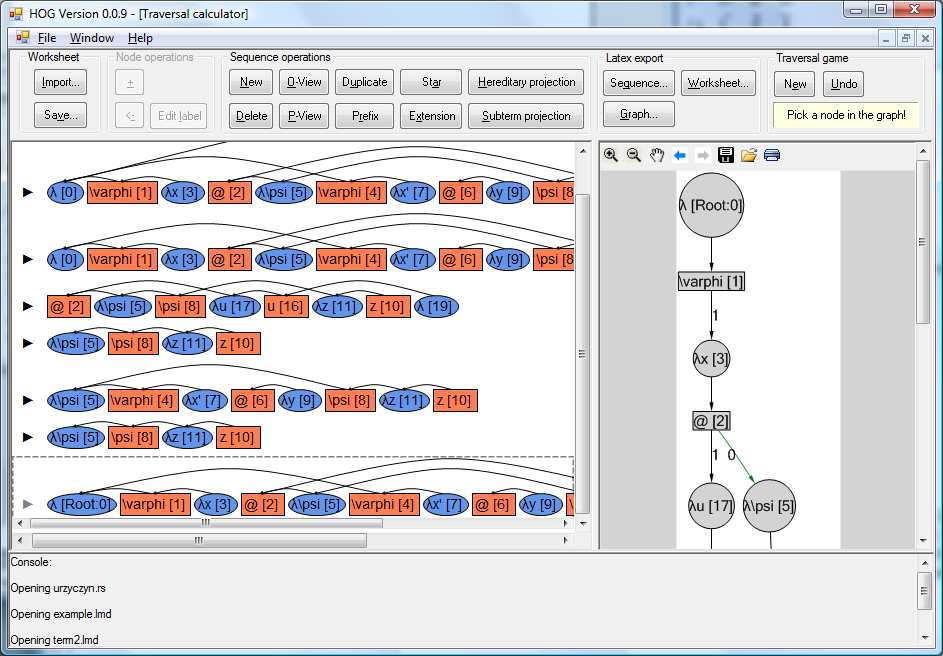
\includegraphics[width=11cm]{sshot.jpg}

}




%%%%%%%%%%%%%%%%%%%%%%%%%%%%%%%%%%%%%%%%%%%%%%%%%

\section{Applications}


\subsection{Higher-order grammars}
\frame{\frametitle{Higher-order grammars}
\emph{Notation for types:} $A_1 \rightarrow (A_2 \rightarrow (\ldots (A_n \rightarrow o)) \ldots )$
is written $(A_1,A_2,\ldots, A_n,o)$.

\begin{itemize}

\item Higher-order grammars used as generators of word languages, trees or graphs  are called \highlight{recursion schemes} (Maslov, 1974).

\item A \highlight{higher-order grammar} is formally given by a tuple
$\langle \Sigma, \mathcal{N}, \mathcal{R}, \mathcal{S} \rangle$
(terminals, non-terminals, rewritting rules, starting symbol)

\item Example of a tree-generating order-2 recursion scheme:
\begin{columns}
      \column{.3\textwidth}
$\begin{array}{rll}
  S & \rightarrow & H \, a\\
  H \, z^o & \rightarrow & F \, (g \,
  z)\\
  F \, \phi^{(o, o)} & \rightarrow & \phi \, (\phi \, (F \, h))\\
\end{array}$
      \column{.3\textwidth}
\begin{tikzpicture}[baseline=(root.base),level distance=5mm,inner ysep=0.5mm,sibling distance=10mm]
 \node (root) {$g$}
    child {node {$a$}}
    child {node {$g$}
        child { node{$a$} }
        child { node{$h$}
                child { node{$h$}
                        child { node{$\vdots$} }
                }
        }
    } ;
\end{tikzpicture}
\end{columns}
Non-terminals: $S :o$, $H:(o,o)$ and $F:((o,o),o)$. Terminals: $a:o$ and $g,h:(o,o)$.
\end{itemize}
}

\frame{
\frametitle{Tree generating HO-PDA}
Higher-order pushdown automata (HOPDA)
generalize PDA to nested stacks. An 1-PDA is a standard PDA. An order $n$-HOPDA manipulates a stack with $n$ levels of nesting.

The transitions are of the following kinds:
\begin{itemize}
    \item $push_1 a$: push the element $a$ on the top level $1$-stack;
    \item $pop_1$: pop the top element of the top level $1$-stack;
    \item $push_n$, $n>1$: duplicate the top level $n-1$-stack;
    \item $pop_n$, $n>1$: delete the top level $n-1$-stack.
\end{itemize}
Additionally, since we use HOPDA to generate a tree, we have:
\begin{itemize}
  \item $emit_f (q_1, \ldots, q_k)$, for each node-constructor $f:o^k\typear \in \Sigma$.
\end{itemize}

\begin{theorem}
For generating word or tree languages, order-$n$ pushdown automata
are equivalent to order-$n$ \highlight{safe} grammars [Damm82,KNU02].
\end{theorem}
}

\frame{
\frametitle{Collapsible PDA}

What is the automaton equivalent of unrestricted grammars?
\pause

\begin{itemize}
\item Answer: Collapsible Pushdown Automaton CPDA [Hague,Murawski,Ong,Serre, LICS08]:
\begin{itemize}
    \item it is an extension of HO-PDA where each symbol in the stack can have a pointer to a sub-stack occurring underneath it;
    \item it can ``collapse'' the stack by following the pointer associated to the top element.
\end{itemize}

\item There is a transformation from HORS to CPDA and reciprocally.

\item The first transformation is based on the traversal framework:
\begin{enumerate}[1.]
  \item compute the computation graph of the HORS by taking the $\eta$-long nf of each grammar rule;
  \item construct a CPDA ``simulating'' the HORS by calculating the traversal of its computation graph.
\end{enumerate}
\pause
\item Tool demo...
\end{itemize}

}

\subsection{Other applications}
\frame{\frametitle{Other applications, related works}

\begin{itemize}
\item \highlight{Verification:}  Knapik {\it et.\ al.} (2002) showed that \highlight{MSO model checking} for trees generated by HORS
 of any order and verifying the \highlight{safety restriction} (a syntactic restriction that constrains the occurrences of variables according to their orders) is decidable.

    Using the notions of computation tree/traversal Ong was able to show (LICS06) that this result still holds in the unrestricted case.
%\item Ong introduced computation trees in LICS2006 to prove decidability of MSO theory on infinite trees
%generated by higher-order grammars.

\pause

\item Studying the effect of syntactic restrictions on the game semantics model.
 \eg\ One can show that \highlight{pointers are uniquely recoverable} in the game denotation of terms satisfying the safety restriction.
\pause

\end{itemize}

\highlight{Related works:}

\begin{itemize}
\item Stirling recently proved decidability of higher-order pattern matching with a game-semantic approach
 relying on equivalent notions of computation tree and traversal.
\end{itemize}
}



%%%%%%%%%%%%%%%%%%%%%%%%%%%%%%%%%%%%%%%%%%%%%%%%%
%\subsection{Simply Typed \texorpdfstring{$\lambda$}{Lambda}-Calculus}
%\frame{\frametitle{Simply Typed $\lambda$-Calculus}
%\begin{itemize}
%\item \highlight{Simple types} $A := o\ |\ A \rightarrow A$.
%%We write $(A_1,\ldots, A_n)$ for $A_1\rightarrow \ldots \rightarrow A_n$.
%
%\item The \highlight{order} of a type is given by $\textsf{order}(o) = 0$,
%$\textsf{order}(A \rightarrow B) = \max(\textsf{order}(A) + 1, \textsf{order}(B))$.
%
%
%\end{itemize}
%}
%



\section{Future Works}
\frame{ \frametitle{Future Works}

%\highlight{Future works:}
\begin{itemize}
\item Implement other transformations: from CPDA to HORS and from safe HORS to PDA.
\item Implement the MSO decision procedure.
\item Application to implicit complexity: can we obtain space-complexity characterizations by analyzing the length of the traversals? (See Kazushige Terui's work.)
\end{itemize}


}

\begin{frame} \frametitle<presentation>{Bibliography}

  \begin{thebibliography}{10}
  \beamertemplatearticlebibitems
    \bibitem{abramsky:game-semantics-tutorial}
    Samson Abramsky and Guy McCusker.
    \newblock Game semantics, Lecture notes.
    \newblock In {\em Proceedings of the 1997 Marktoberdorf Summer School}. Springer-Verlag, 1998.

%    \bibitem{safety-mirlong2004}
%    Klaus Aehlig, Jolie~G. de~Miranda, and C.-H.~Luke Ong.
%    \newblock Safety is not a restriction at level 2 for string languages.
%    \newblock Technical report. University of Oxford, 2004.

    \bibitem{hague-sto07}
    M.~Hague, A.S.~Murawski, C.-H.~L. Ong and O.~Serre.
    \newblock Collapsible pushdown automata and recursive schemes.
    \newblock To appear, LICS2008.

    \bibitem{OngLics2006}
    C.-H.~Luke Ong.
    \newblock On model-checking trees generated by higher-order recursion schemes.
    \newblock In {\em Proceedings of LICS.} Computer Society Press, 2006.

    \bibitem{DBLP:conf/icalp/Stirling06}
    Colin Stirling
    \newblock A Game-Theoretic Approach to Deciding Higher-Order Matching.
    \newblock In {\em Proceedings of ICALP.} Springer, 2006.

  \end{thebibliography}
\end{frame}




\note{
\begin{itemize}
\item nPDA = finite state machines + order n stack
\item For words: 1PDA recognizes context-free language.
        and 0PDA = recognizes regular language.
\item MSO is very expressive: more than the modal mu-calculus (into which LTL CTL CTL* can be embedded.
But over trees, MSO and modal mu-calculus are equi-expressive.)
\item [Caucal02] Graphs generated by safe grammars have a decidable MSO theory.
\item [HMOS06] Caucal's result does not extend to unsafe grammars.
However deciding $\mu$-calculus theories is $n$-EXPTIME complete.
\end{itemize}
}


\end{document}

\def\toolname{HOG}

\pstrSetArrowColor{black}

\title{\texorpdfstring{A Concrete Presentation of Game Semantics}{A Concrete Presentation of Game Semantics}}

\author[W. Blum, C.-H. L. Ong]{\texorpdfstring{\\ William Blum\\ \ \\
 Joint work with C.-H. Luke Ong}{William Blum}}


\institute[Oxford University -- Edinburgh University]{School of Informatics, University of Edinburgh -- Oxford University Computing Laboratory}

\date{\small \color{red}{Galop 2008, 5 April 2008}}


\begin{document}

\frame{\titlepage}

\frame{\frametitle{Overview}
\begin{itemize}
  \item
Game-semantic model are \highlight{abstract} \ie independent of the syntax of the denotated term. We give here a \highlight{concrete} \ie syntactic representation of game semantics where:
\begin{itemize}
\item The arena game is incarnated by some abstract syntax tree of the term.
\item Plays become traversals over this tree.
\end{itemize}


\item A ``Correspondence Theorem'' establishes the relationship between the game-semantic and traversal models.

\item We developed the tool \toolname\ to illustrate this correspondence.

\item Example of application:
computing infinite trees generated by \emph{higher-order recursion scheme}.
\end{itemize}



%We briefly present a new representation theory for game semantics which is very concrete: instead of playing in an arena game in which P plays the innocent strategy given by a term, the same game is played out over (a souped up version of) the abstract syntax tree of the term itself. The plays that are thus traced out are called \highlight{traversals}. More abstractly, traversals are the justified sequences that are obtained by performing parallel-composition \emph{less} the hiding. After stating and explaining a number of Path-Traversal Correspondence Theorems, we present a tool for game semantics based on the new representation.

}


%\section<presentation>*{Outline}
\begin{frame}
  \frametitle{Outline}
  \tableofcontents
\end{frame}

\AtBeginSection[] {
   \begin{frame}
     \frametitle{Outline}
     \tableofcontents[currentpart,currentsection]
   \end{frame}
 }


%%%%%%%%%%%%%%%%%%%%%%%%%%%%%%%%%%%%%%%%%%%%%%%%%
\section{The correspondence}

\subsection{Game semantics}

%%% The Correspondence in one slide
%\frame{ \frametitle{Correspondence Theorem}
%Let $\vdash M:T$ be a pure simply typed term.
%
%\begin{itemize}
%\item \highlight{Game-semantics} provides a model of $\lambda$-calculus.
%$M$ is denoted by a strategy $\sem{M}$ on a 2-player game induced by $T$.
%\item A \highlight{strategy} is represented by a set of sequences of moves together with \highlight{links}: each move points
%to a preceding move.
%\pause
%\item \textcolor{DarkGreen}{Computation tree} = canonical tree representation of a term.
%\item \textcolor{DarkGreen}{Traversals $\travset(M)$ } = sequences of nodes with links respecting some formation rules.
%\end{itemize}
%\pause
%
%\begin{block}{The Correspondence Theorem}
%The game semantics of a term can be represented on the computation
%tree:
%$$ \textcolor{DarkGreen}{\travset(M)} \cong \textcolor{blue}{\intersem{M}} $$
%$$ \textcolor{DarkGreen}{Reduction(\travset(M))} \cong \textcolor{blue}{\sem{M}}$$
%where $\textcolor{blue}{\intersem{M}}$ is the revealed game-semantic denotion (i.e. internal moves are uncovered).
%\end{block}
%}

\frame{\frametitle{Game semantics}
 Model of programming languages based on games (Abramsky et al.; Hyland and Ong; Nickau)
\begin{itemize}
\item 2 players: \highlight{O}pponnent (system) and \highlight{P}roponent (program)
\item The term type induces an \highlight{arena} defining the possible moves
$\sem{\nat} = 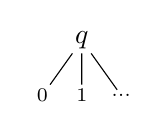
\begin{tikzpicture}[baseline=(root.base),level distance=7mm,inner ysep=0.5mm,sibling distance=5mm]
 \node (root) {$q$}
    child {node {$\scriptstyle 0$}}
    child {node {$\scriptstyle 1$}}
    child {node {$\scriptstyle \ldots$}}
;
\end{tikzpicture}$
\hspace{2cm}
$\sem{\nat \rightarrow \nat} = 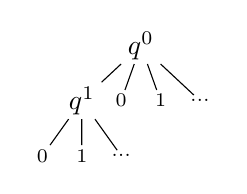
\begin{tikzpicture}[baseline=(root.base),level distance=7mm,inner ysep=0.5mm,sibling distance=5mm]
 \node (root) {$q^0$}
    child{
      node{$q^1$}
      child{node {$\scriptstyle 0$} }
      child{node {$\scriptstyle 1$} }
      child {node {$\scriptstyle \ldots$}}
    }
    child {node {$\scriptstyle 0$}}
    child {node {$\scriptstyle 1$}}
    child {node {$\scriptstyle \ldots$}}
;
\end{tikzpicture}$
\item \highlight{Play} = sequence of moves played alternatively by O and P with justification pointers.
\item \highlight{Strategy for P} = prefix-closed set of plays. $s  a  b$ in the strategy means that
P should respond $b$ when O plays $a$ in position $s$.
\item The \highlight{denotation} of a term $M$, written $\sem{M}$, is a strategy for P.
\item $\sem{ 7 : \nat} = \{ \epsilon, q, q\ 7 \}$\\
$\sem{ \pcfsucc : \nat \rightarrow \nat} = Pref( \{ q^0 q^1 n ( n+1)
\ | \ n \in \nat \} )$
\item Compositionality: $\sem{ \pcfsucc\  7} = \sem{ \pcfsucc } ; \sem{7}$
\end{itemize}
}

\frame{
\frametitle{Game semantics: composition}

\begin{itemize}
    \item Composition is done by CSP-composition + hiding:
If $\sigma : A \typear B$ and $\mu : B \typear C$ then
$$\mbox{`` }\sigma ; \mu =  (\sigma \| \mu ) \filter A,C \mbox{ ''}$$
\pause

    \item  The \highlight{fully revealed} game denotation, written $\revsem{M}$, to denote
    the set of plays obtained when hiding is never performed during composition.

    \item  The \highlight{syntactically-revealed} denotation, written $\syntrevsem{M}$, hides certain moves during composition:
in the denotation of $\revsem{x N_1\ldots N_p}$ for some variable $x$, the internal moves of $N_1$,\ldots,$N_p$ are preserved while the internal moves produced by the copy-cat projection strategy denoting $x$ are omitted.
\end{itemize}



}

\def\highlightat#1#2{\temporal<#1>{#2}{\underline{#2}}{\textcolor{blue}{#2}}}

\subsection{Computation tree}
\frame{ \frametitle{Computation tree}

We fix a simply-typed term $\Gamma \vdash M: T$.

\highlight{\it Computation tree} of $M$ is the AST of its $\eta$-long normal form.
\begin{itemize}
\item The \highlight{$\eta$-expansion} of $M:A\typear B$ is $\lambda x:A . Mx :A\typear B$.
\item The \highlight{$\eta$-long normal form} of $M$ is obtained
by hereditarily $\eta$-expanding every subterm of $M$ occurring at an operand position or as the body of a $\lambda$-abstraction.
\end{itemize}

Example:
$$h: o\typear o \vdash \lambda f^{o \typear o} .
(\lambda u^{o \typear o} . u) h : (o \typear o) \typear
o \typear o$$

\begin{columns}
\column{6cm}
Its $\eta$-long normal is
\begin{align*}
h: o \typear o &\vdash  \lambda f^{o \typear o} z^o . \\
&\qquad(\lambda u^{o \typear o} v^o . u (\lambda.v)) \\
&\qquad(\lambda y^o. h y) \\
&\qquad(\lambda.z) \\
&: (o \typear o) \typear o \typear o
\end{align*}

\column{4cm}
The computation tree is:
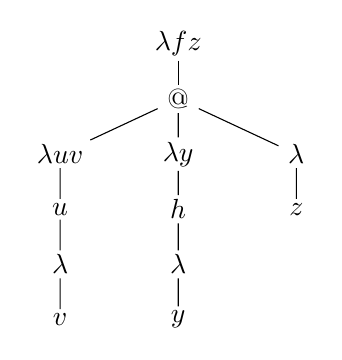
\begin{tikzpicture}[level distance=7mm,inner ysep=0.5mm]
 \node {$\lambda f z$}
    child {
        node {@}
        child {
            node {$\lambda u v$}
            child{
                node{$u$}
                child {
                    node{$\lambda$}
                    child {
                        node{$v$}
                    }
                }
            }
        }
        child {
            node {$\lambda y$}
            child{
                node {$h$}
                child{
                    node {$\lambda$}
                    child { node {$y$} }
                }
            }
        }
        child {
            node {$\lambda$}
            child{ node {$z$} }
            }
        };
\end{tikzpicture}
\end{columns}
}


\frame{
\frametitle{Justified sequence}

\begin{itemize}
\item  We define an \highlight{enabling relation} $\vdash$ on the set of nodes:
\begin{itemize}
  \item a bound variable is enabled by its binder;
  \item a free variable is enabled by the root $\theroot$;
  \item a lambda node  is enabled by its parent node;
  \item an @-node has no enabler.
\end{itemize}

\item A \highlight{justified sequence} is a sequence of nodes such that all the non @-nodes have a justification pointer respecting the relation $\vdash$.

\item  The analogy with game semantics is:
\begin{itemize}
\item $\lambda$-nodes $\equiv$ O-moves
\item @-nodes and variable-nodes $\equiv$ P-moves
\end{itemize}

We can define notions of P-view and O-view, alternation, P-visibility, O-visibility.


\item The computation will be described by a set $\travset(M)$ of justified sequences called \highlight{traversals}.
\end{itemize}
}




\frame{
\frametitle{Traversals rules}
The set $\travset(M)$ is given by induction over the rules:
%\begin{FramedTable}
%\noindent {\bf Initialization rules}
\begin{itemize}[]
\item\rulenamet{Empty} $\epsilon \in\travset(M)$
\item \rulenamet{Root} $\theroot \in \travset(M)$
%\end{itemize}
%\noindent {\bf Structural rules}
%\begin{itemize}[]
    \item \rulenamet{Lam} $t \cdot \lambda \overline{\xi} \in\travset(M) \implies t \cdot \lambda \overline{\xi} \cdot n \in\travset(M)$ where $n$
        is $\lambda \overline{\xi}$'s child and is justified by the only occurrence of
        its enabler in the P-view
    \item \rulenamet{App}  $t \cdot @ \in\travset(M) \implies$ \Pstr[0.4cm]{t \cdot (m) @  \cdot (n-m,40:0) n} $\in\travset(M)$.
%\end{itemize}
%\emph{\bf Input-variable rules}
%\begin{itemize}[]
\item \rulenamet{ContextVar} $t\cdot x\in\travset(M)$, $x\in N^{\theroot\vdash}_{\sf var}$ $\implies$
$t \cdot x \cdot n \in\travset(M)$
for any $\lambda$-node $n$ justified by some
occurrence of its parent node in $\oview{t}$.

%\item \rulenamet{ContextValue} If $t_1
%\cdot x \cdot t_2 \in\travset(M)$ with pending node $x \in
%N_{\sf var}^{\theroot\vdash}$ then so is \Pstr[0.5cm]{t_1 \cdot
%(x){x} \cdot t_2 \cdot (xv-x,38:v){v_x} } for all $v \in
%\mathcal{D}$.
%\end{itemize}
%\emph{\bf Copy-cat rules}
%\begin{itemize}[]
\item\rulenamet{Var}
\Pstr[0.2cm]{t \cdot (n){n} \cdot (lx){\lambda \overline{x}}
    \ldots (x-lx,40:i){x_i} } $\in\travset(M)$, $x_i \in
    N_{\sf var}^{@\vdash} \implies$  \Pstr[0.5cm]{ t \cdot
(n){n} \cdot (lx){\lambda \overline{x}}  \ldots (x-lx,25:i){x_i}
    \cdot (letai-n,32:i){\lambda \overline{\eta_i}}} $\in\travset(M)$.
%\item\rulenamet{Value}
%  If \Pstr{t \cdot (m){m} \cdot (n){n}  \ldots
%(vn-n,50:v){v}_{n} } $\in\travset(M)$ where $n\in N$ then
%\Pstr[0.6cm]{t \cdot (m){m} \cdot (n){n} \ldots
%(vn-n,50:v){v}_{n} \cdot (vm-m,45:v){v}_m} $\in\travset(M)$.
\end{itemize}
%\caption[Traversal rules for the simply-typed
%lambda-calculus]{Traversal rules for the simply-typed
%$\lambda$-calculus.}
%\label{tab:trav_rules}
%\end{FramedTable}

}


\frame{
\frametitle{Example of traversal}


\begin{center}
%\begin{columns}
%\column{6cm}
%\column{3.5cm}
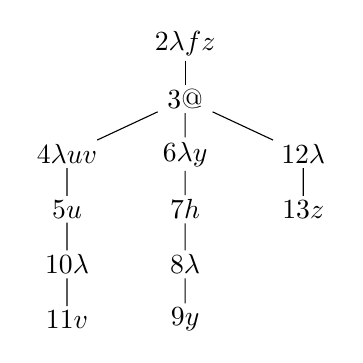
\begin{tikzpicture}[level distance=7mm,inner ysep=0.5mm]
 \node {\highlightat{2}{$\lambda f z$}}
    child {
        node {\highlightat{3}{@}}
        child {
            node {\highlightat{4}{$\lambda u v$}}
            child{
                node{\highlightat{5}{$u$}}
                child {
                    node{\highlightat{10}{$\lambda$}}
                    child {
                        node{\highlightat{11}{$v$}}
                    }
                }
            }
        }
        child {
            node {\highlightat{6}{$\lambda y$}}
            child{
                node {\highlightat{7}{$h$}}
                child{
                    node {\highlightat{8}{$\lambda$}}
                    child { node {\highlightat{9}{$y$}} }
                }
            }
        }
        child {
            node {$\highlightat{12}{\lambda}$}
            child{ node {\highlightat{13}{$z$}} }
            }
        };
\end{tikzpicture}
%\end{columns}
\end{center}

\setbox0=\hbox{$\textcolor{blue}{
\pstr{\only<2->{\nd t= (n0){\lambda f z}}
        \only<3->{\nd\cdot (n1){@}}
        \only<4->{\nd\cdot (n2-n1){\lambda u v}}
        \only<5->{\nd\cdot (n3-n2){u}}
        \only<6->{\nd\cdot (n4-n1){\lambda y}}
        \only<7->{\nd\cdot (n5-n0){h}}
        \only<8->{\nd\cdot (n6-n5){\lambda }}
        \only<9->{\nd\cdot (n7-n4){y}}
        \only<10->{\nd\cdot (n8-n3){\lambda }}
        \only<11->{\nd\cdot (n9-n2){v}}
        \only<12->{\nd\cdot (n10-n1){\lambda }}
        \only<13->{\nd\cdot (n11-n0){z}}
}}$}
\ht0 2cm\box0 % Make sure the height of box containing the traversal remains constant across the different generated slides

}

\frame{
\frametitle{Operations on traversals}
$\pstr{\nd t= (n0){\lambda f z}
        \nd\cdot (n1){@}
        \nd\cdot (n2-n1){\lambda u v}
        \nd\cdot (n3-n2){u}
        \nd\cdot (n4-n1){\lambda y}
        \nd\cdot (n5-n0){h}
        \nd\cdot (n6-n5){\lambda }
        \nd\cdot (n7-n4){y}
        \nd\cdot (n8-n3){\lambda }
        \nd\cdot (n9-n2){v}
        \nd\cdot (n10-n1){\lambda }
        \nd\cdot (n11-n0){z}
}$
\vspace*{0.4cm}
\begin{itemize}
\item The \highlight{reduction of a traversal} is obtained by keeping only
the occurrences hereditarily justified by the root:
$$\color{red}{ \Pstr[0.7cm]{t \upharpoonright r = (n0){\lambda f z}\ (n1-n0){h}\ (n2-n1){\lambda }\ (n3-n0){z} } }$$
\pause

\item  \highlight{\it @-nodes removal:}
$$\Pstr[0.5cm]{ t - @ = (n0){\lambda f z}\ (n1-n0){\lambda u v}\ (n2-n1){u}\ (n3-n0){\lambda y}\ (n4-n0){h}\ (n5-n4){\lambda }\ (n6-n3){y}\ (n7-n2){\lambda }\ (n8-n1){v}\ (n9-n0){\lambda }\ (n10-n0){z}}$$
\end{itemize}

}


\subsection{The Correspondence Theorem}
\frame{ \frametitle{The Correspondence Theorem}
\begin{block}{}
Let $M$ be a simply typed term of type $T$. There exists a partial function $\textcolor{DarkGreen}{\varphi}$
from the nodes of the \highlight{computation tree} to the
moves of the \highlight{arena} $\sem{T}$ such that
$$ \textcolor{DarkGreen}{\varphi}  : \travset(M)^{-@} \textcolor{DarkGreen}{\stackrel{\cong}{\longrightarrow}}
\syntrevsem{M} $$
$$ \textcolor{DarkGreen}{\varphi}  : \travset(M)^{\upharpoonright r}  \textcolor{DarkGreen}{\stackrel{\cong}{\longrightarrow}} \sem{M} \ .$$
\end{block}
where
\begin{itemize}
\item $\highlight{\travset(M)}$ = set of traversals of the computation tree of $M$
\item $\highlight{\travset(M)^{\upharpoonright r}} = \{ t \upharpoonright r \ | \  t \in {\travset(M)} \}$
\item $\highlight{\travset(M)^{-@}} = \{ t - @ \ | \  t \in {\travset(M)} \}$
\item $\highlight{\sem{M}}$ = game-semantic denotation of $M$
\item $\highlight{
\syntrevsem{M}}$ = syntactically-revealed denotion of $M$.
\end{itemize}

}


\frame{ \frametitle{More correspondences}
\begin{center}
\begin{tabular}{c|c}
Computation tree notions & Game-semantic equivalents \\ \hline \hline \\
computation tree & arena(s) \\ \\
traversal & uncovered play \\ \\
reduced traversal & play \\ \\
path in the computation tree & P-view of an uncovered play
\end{tabular}
\end{center}
}


\subsection{Example}
\frame{\frametitle{Example:
 $o \typear o \vdash \lambda f^{o \typear o} .
(\lambda u^{o \typear o} . u) h : (o \typear o) \typear
o \typear o$}

Left: computation tree. Right: arena.
\begin{center}
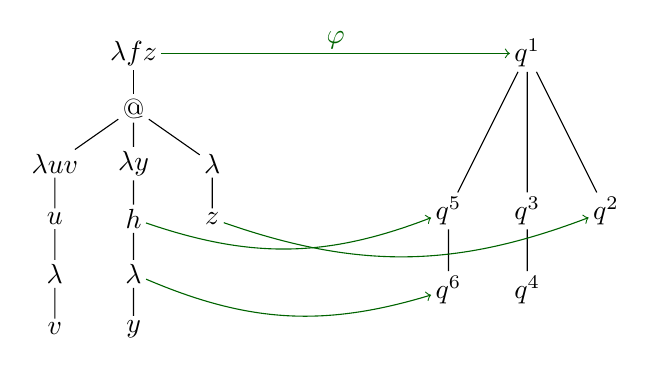
\begin{tikzpicture}[level distance=7mm,inner ysep=0.5mm,inner xsep=0.5mm,sibling distance=10mm]
%\color{blue}
\node (root) {$\lambda f z$}
    child{
      node{$@$}
          child{
            node {$\lambda u v$}
            child{
              node (u) {$u$}
              child{
                node (lmd) {$\lambda$}
                child{
                  node {$v$}
                }
              }
            }
          }
          child{
            node {$\lambda y$}
            child{
                node (h) {$h$}
                child{
                  node (h1) {$\lambda$}
                  child{
                    node {$y$}
                  }
                }
            }
          }
          child{
            node {$\lambda$}
            child{
              node (z) {$z$}
            }
          }
      }
;
%\color{red}
\draw +(5,0) node (q1) {$q^1$}
    [level distance=20mm]
      child{
        node (q5) {$q^5$}
        [level distance=10mm]
        child{ node (q6) {$q^6$} }
      }
      child{
        node (q3) {$q^3$}
        [level distance=10mm]
        child{ node (q4) {$q^4$} }
      }
      child{ node (q2) {$q^2$} }
;
\color{DarkGreen}
\draw[->] (root) -- node[above] {$\varphi$} (q1);
\draw[->] (h) to [bend right=20]  (q5);
\draw[->] (h1) to [bend right=20]  (q6);
\draw[->] (z) to [bend right=20]  (q2);
\end{tikzpicture}
\end{center}
\begin{itemize}
\item $\pstr{\nd t= (n0){\lambda f z}
        \nd\cdot (n1){@}
        \nd\cdot (n2-n1,35){\lambda u v}
        \nd\cdot (n3-n2,35){u}
        \nd\cdot (n4-n1,35){\lambda y}
        \nd\cdot (n5-n0,35){h}
        \nd\cdot (n6-n5,35){\lambda }
        \nd\cdot (n7-n4,35){y}
        \nd\cdot (n8-n3,35){\lambda }
        \nd\cdot (n9-n2,35){v}
        \nd\cdot (n10-n1,35){\lambda }
        \nd\cdot (n11-n0,35){z}
}$

\item $\Pstr{\pview{t} = (q1){\lambda f z} \cdot (n2){@}
\cdot (n9-n2,35){\lambda}
\cdot (q2-q1,35){z}}$

\item
$
\textcolor{DarkGreen}{
\varphi (} %\textcolor{blue}
{t \upharpoonright r}
\textcolor{DarkGreen}{)} = \textcolor{DarkGreen}{\varphi (}
\textcolor{blue}{
\Pstr[70mm]{ (q1){\lambda f z}
            \cdot (q3-q1){h}
            \cdot (q4-q3){\lambda}
            \cdot (q2-q1){z} }
}
\textcolor{DarkGreen}{)} = %\textcolor{red}
{
\Pstr[70mm]{
    (q1){q}^1\
    (q5-q1){q}^5\
    (q6-q3){q}^6\
    (q2-q1){q}^2
}}
\in %\textcolor{red}
{\sem{M}}.
$

\end{itemize}
}



\begingroup
\newcommand\sigcol[1]{{\color{blue} #1}}
\newcommand\mucol[1]{{\color{red} #1}}
\newcommand\mynodeex[2]{\node[name=#1]{$#2$};}

\subsection{Composition}
\begin{frame}[fragile]
\frametitle{Composition}

Take $\sigcol{\sigma} = \sem{ \vdash \sigcol{\lambda x^o v^o .x} : o\typear (o,o)}$
 and  $\mucol{\mu} = \sem{ \vdash \mucol{\lambda y^{(o,o)} \varphi^{((o,o),o)}. \varphi (\lambda u^o . y~u)} : (o,o) \typear (((o,o),o),o)}$.

We then have $\sigcol{\sigma} \fatcompos \mucol{\mu} = \sem{ \lambda x \varphi. \varphi (\lambda u . x) : o \typear (((o,o),o),o)}$.
\bigskip

\begin{tikzpicture}
  [every node/.style={anchor=base}]
  \matrix [matrix of nodes]
  {
    o & $\stackrel{\sigcol{\sigma}}\longrightarrow$ & (o,& o) & $\stackrel{\mucol{\mu}}\longrightarrow$ &  (((o,&o),&o), & o) \\
&&&&&&&&\mynodeex{n0}{\lambda x \varphi \omove  \mucol {\lambda y \varphi}}\\
&&&&&&&\mynodeex{n1}{\varphi  \pmove \mucol \varphi}\\
&&&&&&\mynodeex{n2}{\lambda u \omove  \mucol {\lambda u}} \\
&&&  \mynodeex{n3}{\sigcol {\lambda x v} \opmove \mucol y} \\
\mynodeex{n4}{x \pmove \sigcol x}\\
  };
\draw[->] (n4) .. controls +(60:1cm) and +(-1,0) .. (n0.west);
\draw[->] (n2) .. controls +(60:0.2cm) and +(-0.4cm,0) .. (n1.west);
\draw[->] (n1) .. controls +(60:0.2cm) and +(-0.4cm,0) .. (n0.west);
\draw[->] (n3) .. controls +(30:1cm) and +(-1,0) .. (n0.west);
\draw[->] (n4) .. controls +(30:1cm) and +(-1,0) .. (n3.west);
\end{tikzpicture}
\end{frame}
\endgroup


\subsection{Demo}
\frame{\frametitle{Tool demo}
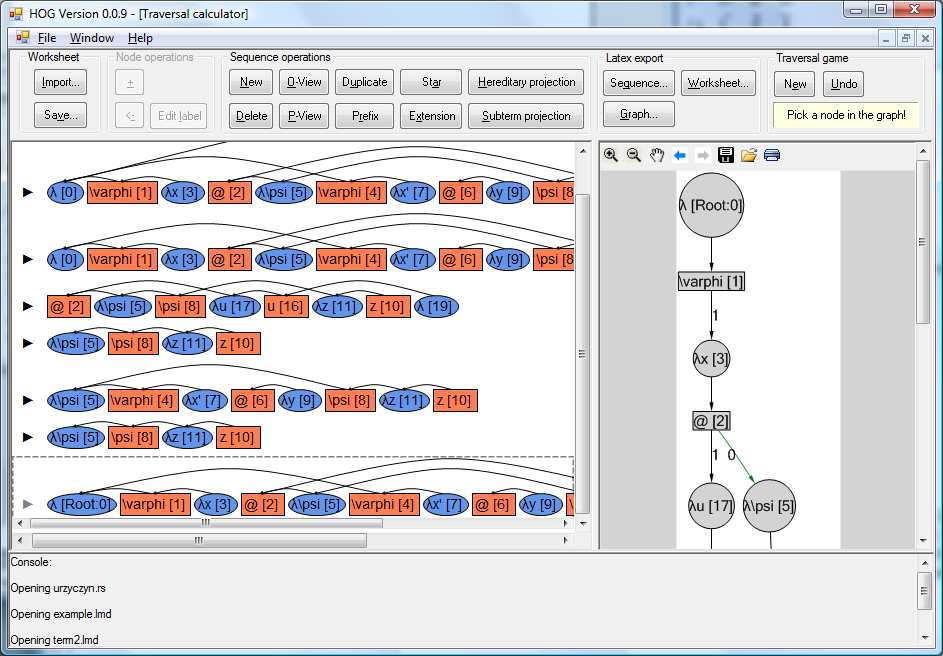
\includegraphics[width=11cm]{sshot.jpg}

}




%%%%%%%%%%%%%%%%%%%%%%%%%%%%%%%%%%%%%%%%%%%%%%%%%

\section{Applications}


\subsection{Higher-order grammars}
\frame{\frametitle{Higher-order grammars}
\emph{Notation for types:} $A_1 \rightarrow (A_2 \rightarrow (\ldots (A_n \rightarrow o)) \ldots )$
is written $(A_1,A_2,\ldots, A_n,o)$.

\begin{itemize}

\item Higher-order grammars used as generators of word languages, trees or graphs  are called \highlight{recursion schemes} (Maslov, 1974).

\item A \highlight{higher-order grammar} is formally given by a tuple
$\langle \Sigma, \mathcal{N}, \mathcal{R}, \mathcal{S} \rangle$
(terminals, non-terminals, rewritting rules, starting symbol)

\item Example of a tree-generating order-2 recursion scheme:
\begin{columns}
      \column{.3\textwidth}
$\begin{array}{rll}
  S & \rightarrow & H \, a\\
  H \, z^o & \rightarrow & F \, (g \,
  z)\\
  F \, \phi^{(o, o)} & \rightarrow & \phi \, (\phi \, (F \, h))\\
\end{array}$
      \column{.3\textwidth}
\begin{tikzpicture}[baseline=(root.base),level distance=5mm,inner ysep=0.5mm,sibling distance=10mm]
 \node (root) {$g$}
    child {node {$a$}}
    child {node {$g$}
        child { node{$a$} }
        child { node{$h$}
                child { node{$h$}
                        child { node{$\vdots$} }
                }
        }
    } ;
\end{tikzpicture}
\end{columns}
Non-terminals: $S :o$, $H:(o,o)$ and $F:((o,o),o)$. Terminals: $a:o$ and $g,h:(o,o)$.
\end{itemize}
}

\frame{
\frametitle{Tree generating HO-PDA}
Higher-order pushdown automata (HOPDA)
generalize PDA to nested stacks. An 1-PDA is a standard PDA. An order $n$-HOPDA manipulates a stack with $n$ levels of nesting.

The transitions are of the following kinds:
\begin{itemize}
    \item $push_1 a$: push the element $a$ on the top level $1$-stack;
    \item $pop_1$: pop the top element of the top level $1$-stack;
    \item $push_n$, $n>1$: duplicate the top level $n-1$-stack;
    \item $pop_n$, $n>1$: delete the top level $n-1$-stack.
\end{itemize}
Additionally, since we use HOPDA to generate a tree, we have:
\begin{itemize}
  \item $emit_f (q_1, \ldots, q_k)$, for each node-constructor $f:o^k\typear \in \Sigma$.
\end{itemize}

\begin{theorem}
For generating word or tree languages, order-$n$ pushdown automata
are equivalent to order-$n$ \highlight{safe} grammars [Damm82,KNU02].
\end{theorem}
}

\frame{
\frametitle{Collapsible PDA}

What is the automaton equivalent of unrestricted grammars?
\pause

\begin{itemize}
\item Answer: Collapsible Pushdown Automaton CPDA [Hague,Murawski,Ong,Serre, LICS08]:
\begin{itemize}
    \item it is an extension of HO-PDA where each symbol in the stack can have a pointer to a sub-stack occurring underneath it;
    \item it can ``collapse'' the stack by following the pointer associated to the top element.
\end{itemize}

\item There is a transformation from HORS to CPDA and reciprocally.

\item The first transformation is based on the traversal framework:
\begin{enumerate}[1.]
  \item compute the computation graph of the HORS by taking the $\eta$-long nf of each grammar rule;
  \item construct a CPDA ``simulating'' the HORS by calculating the traversal of its computation graph.
\end{enumerate}
\pause
\item Tool demo...
\end{itemize}

}

\subsection{Other applications}
\frame{\frametitle{Other applications, related works}

\begin{itemize}
\item \highlight{Verification:}  Knapik {\it et.\ al.} (2002) showed that \highlight{MSO model checking} for trees generated by HORS
 of any order and verifying the \highlight{safety restriction} (a syntactic restriction that constrains the occurrences of variables according to their orders) is decidable.

    Using the notions of computation tree/traversal Ong was able to show (LICS06) that this result still holds in the unrestricted case.
%\item Ong introduced computation trees in LICS2006 to prove decidability of MSO theory on infinite trees
%generated by higher-order grammars.

\pause

\item Studying the effect of syntactic restrictions on the game semantics model.
 \eg\ One can show that \highlight{pointers are uniquely recoverable} in the game denotation of terms satisfying the safety restriction.
\pause

\end{itemize}

\highlight{Related works:}

\begin{itemize}
\item Stirling recently proved decidability of higher-order pattern matching with a game-semantic approach
 relying on equivalent notions of computation tree and traversal.
\end{itemize}
}



%%%%%%%%%%%%%%%%%%%%%%%%%%%%%%%%%%%%%%%%%%%%%%%%%
%\subsection{Simply Typed \texorpdfstring{$\lambda$}{Lambda}-Calculus}
%\frame{\frametitle{Simply Typed $\lambda$-Calculus}
%\begin{itemize}
%\item \highlight{Simple types} $A := o\ |\ A \rightarrow A$.
%%We write $(A_1,\ldots, A_n)$ for $A_1\rightarrow \ldots \rightarrow A_n$.
%
%\item The \highlight{order} of a type is given by $\textsf{order}(o) = 0$,
%$\textsf{order}(A \rightarrow B) = \max(\textsf{order}(A) + 1, \textsf{order}(B))$.
%
%
%\end{itemize}
%}
%



\section{Future Works}
\frame{ \frametitle{Future Works}

%\highlight{Future works:}
\begin{itemize}
\item Implement other transformations: from CPDA to HORS and from safe HORS to PDA.
\item Implement the MSO decision procedure.
\item Application to implicit complexity: can we obtain space-complexity characterizations by analyzing the length of the traversals? (See Kazushige Terui's work.)
\end{itemize}


}

\begin{frame} \frametitle<presentation>{Bibliography}

  \begin{thebibliography}{10}
  \beamertemplatearticlebibitems
    \bibitem{abramsky:game-semantics-tutorial}
    Samson Abramsky and Guy McCusker.
    \newblock Game semantics, Lecture notes.
    \newblock In {\em Proceedings of the 1997 Marktoberdorf Summer School}. Springer-Verlag, 1998.

%    \bibitem{safety-mirlong2004}
%    Klaus Aehlig, Jolie~G. de~Miranda, and C.-H.~Luke Ong.
%    \newblock Safety is not a restriction at level 2 for string languages.
%    \newblock Technical report. University of Oxford, 2004.

    \bibitem{hague-sto07}
    M.~Hague, A.S.~Murawski, C.-H.~L. Ong and O.~Serre.
    \newblock Collapsible pushdown automata and recursive schemes.
    \newblock To appear, LICS2008.

    \bibitem{OngLics2006}
    C.-H.~Luke Ong.
    \newblock On model-checking trees generated by higher-order recursion schemes.
    \newblock In {\em Proceedings of LICS.} Computer Society Press, 2006.

    \bibitem{DBLP:conf/icalp/Stirling06}
    Colin Stirling
    \newblock A Game-Theoretic Approach to Deciding Higher-Order Matching.
    \newblock In {\em Proceedings of ICALP.} Springer, 2006.

  \end{thebibliography}
\end{frame}




\note{
\begin{itemize}
\item nPDA = finite state machines + order n stack
\item For words: 1PDA recognizes context-free language.
        and 0PDA = recognizes regular language.
\item MSO is very expressive: more than the modal mu-calculus (into which LTL CTL CTL* can be embedded.
But over trees, MSO and modal mu-calculus are equi-expressive.)
\item [Caucal02] Graphs generated by safe grammars have a decidable MSO theory.
\item [HMOS06] Caucal's result does not extend to unsafe grammars.
However deciding $\mu$-calculus theories is $n$-EXPTIME complete.
\end{itemize}
}


\end{document}

\def\toolname{HOG}

\pstrSetArrowColor{black}

\title{\texorpdfstring{A Concrete Presentation of Game Semantics}{A Concrete Presentation of Game Semantics}}

\author[W. Blum, C.-H. L. Ong]{\texorpdfstring{\\ William Blum\\ \ \\
 Joint work with C.-H. Luke Ong}{William Blum}}


\institute[Oxford University -- Edinburgh University]{School of Informatics, University of Edinburgh -- Oxford University Computing Laboratory}

\date{\small \color{red}{Galop, 5 April 2008}}


\begin{document}

\frame{\titlepage}

\frame{\frametitle{Overview}
\begin{itemize}
  \item
Game-semantic models are \highlight{abstract} \ie independent of the syntax of the denotated term. We give here a \highlight{concrete} \ie syntactic representation of game semantics where:
\begin{itemize}
\item The arena game is `incarnated' by some abstract syntax tree of the term,
\item Uncovered plays are given by traversals over this tree.
\end{itemize}


\item A ``Correspondence Theorem'' establishes the relationship between the game-semantic and traversal models.

\item The tool \toolname\ illustrates this correspondence.

\item Example of application:
computing infinite trees generated by \emph{higher-order recursion schemes}.
\end{itemize}



%We briefly present a new representation theory for game semantics which is very concrete: instead of playing in an arena game in which P plays the innocent strategy given by a term, the same game is played out over (a souped up version of) the abstract syntax tree of the term itself. The plays that are thus traced out are called \highlight{traversals}. More abstractly, traversals are the justified sequences that are obtained by performing parallel-composition \emph{less} the hiding. After stating and explaining a number of Path-Traversal Correspondence Theorems, we present a tool for game semantics based on the new representation.

}


%\section<presentation>*{Outline}
\begin{frame}
  \frametitle{Outline}
  \tableofcontents
\end{frame}

\AtBeginSection[] {
   \begin{frame}
     \frametitle{Outline}
     \tableofcontents[currentpart,currentsection]
   \end{frame}
 }


%%%%%%%%%%%%%%%%%%%%%%%%%%%%%%%%%%%%%%%%%%%%%%%%%
\section{The correspondence}

\subsection{Game semantics}

%%% The Correspondence in one slide
%\frame{ \frametitle{Correspondence Theorem}
%Let $\vdash M:T$ be a pure simply typed term.
%
%\begin{itemize}
%\item \highlight{Game-semantics} provides a model of $\lambda$-calculus.
%$M$ is denoted by a strategy $\sem{M}$ on a 2-player game induced by $T$.
%\item A \highlight{strategy} is represented by a set of sequences of moves together with \highlight{links}: each move points
%to a preceding move.
%\pause
%\item \textcolor{DarkGreen}{Computation tree} = canonical tree representation of a term.
%\item \textcolor{DarkGreen}{Traversals $\travset(M)$ } = sequences of nodes with links respecting some formation rules.
%\end{itemize}
%\pause
%
%\begin{block}{The Correspondence Theorem}
%The game semantics of a term can be represented on the computation
%tree:
%$$ \textcolor{DarkGreen}{\travset(M)} \cong \textcolor{blue}{\intersem{M}} $$
%$$ \textcolor{DarkGreen}{Reduction(\travset(M))} \cong \textcolor{blue}{\sem{M}}$$
%where $\textcolor{blue}{\intersem{M}}$ is the revealed game-semantic denotion (i.e. internal moves are uncovered).
%\end{block}
%}

\frame{\frametitle{Game semantics}
 Model of programming languages based on games (Abramsky et al.; Hyland and Ong; Nickau)
\begin{itemize}
\item 2 players: \highlight{O}pponnent (system) and \highlight{P}roponent (program)
\item The term type induces an \highlight{arena} defining the possible moves
$\sem{\nat} = 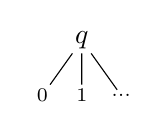
\begin{tikzpicture}[baseline=(root.base),level distance=7mm,inner ysep=0.5mm,sibling distance=5mm]
 \node (root) {$q$}
    child {node {$\scriptstyle 0$}}
    child {node {$\scriptstyle 1$}}
    child {node {$\scriptstyle \ldots$}}
;
\end{tikzpicture}$
\hspace{2cm}
$\sem{\nat \rightarrow \nat} = 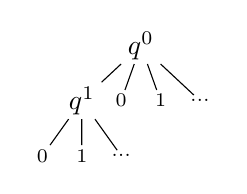
\begin{tikzpicture}[baseline=(root.base),level distance=7mm,inner ysep=0.5mm,sibling distance=5mm]
 \node (root) {$q^0$}
    child{
      node{$q^1$}
      child{node {$\scriptstyle 0$} }
      child{node {$\scriptstyle 1$} }
      child {node {$\scriptstyle \ldots$}}
    }
    child {node {$\scriptstyle 0$}}
    child {node {$\scriptstyle 1$}}
    child {node {$\scriptstyle \ldots$}}
;
\end{tikzpicture}$
\item \highlight{Play} = sequence of moves played alternatively by O and P with justification pointers.
\item \highlight{Strategy for P} = prefix-closed set of plays. $s  a  b$ in the strategy means that
P should respond $b$ when O plays $a$ in position $s$.
\item The \highlight{denotation} of a term $M$, written $\sem{M}$, is a strategy for P.
\item $\sem{ 7 : \nat} = \{ \epsilon, q, q\ 7 \}$\\
$\sem{ \pcfsucc : \nat \rightarrow \nat} = Pref( \{ q^0 q^1 n ( n+1)
\ | \ n \in \nat \} )$
\item Compositionality: $\sem{ \pcfsucc\  7} = \sem{ \pcfsucc } ; \sem{7}$
\end{itemize}
}

\frame{
\frametitle{Game semantics: composition}

\begin{itemize}
    \item Composition is done by CSP-composition + hiding:
If $\sigma : A \typear B$ and $\mu : B \typear C$ then
$$\mbox{`` }\sigma ; \mu =  (\sigma \| \mu ) \filter A,C \mbox{ ''}$$
\pause

    \item  The \highlight{fully revealed} game denotation, written $\revsem{M}$, denotes
    the set of plays obtained by not performing hiding of internal moves during composition.

%    \item  In the \highlight{syntactically-revealed} denotation, written $\syntrevsem{M}$, only certain moves are hidden during composition:
%in the denotation of $\revsem{x N_1\ldots N_p}$ for some variable $x$, the internal moves of $N_1$,\ldots,$N_p$ are preserved while the internal moves produced by the copy-cat projection strategy denoting $x$ are omitted.
\end{itemize}



}

\def\highlightat#1#2{\temporal<#1>{#2}{\underline{#2}}{\textcolor{blue}{#2}}}

\subsection{Computation tree}
\frame{ \frametitle{Computation tree}

We fix a simply-typed term $\Gamma \vdash M: T$.

\highlight{\it Computation tree} of $M$ is the AST of its $\eta$-long normal form.
\begin{itemize}
\item The \highlight{$\eta$-expansion} of $M:A\typear B$ is $\lambda x:A . Mx :A\typear B$.
\item The \highlight{$\eta$-long normal form} of $M$ is obtained
by hereditarily $\eta$-expanding every subterm of $M$ occurring at an operand position or as the body of a $\lambda$-abstraction.
\end{itemize}

Example:
$$\vdash \lambda f^{o \typear o} .
(\lambda u^{o \typear o} . u) f : (o \typear o) \typear
o \typear o$$

\begin{columns}
\column{6cm}
Its $\eta$-long normal form is
\begin{align*}
 &\vdash  \lambda f^{o \typear o} z^o . \\
&\qquad(\lambda u^{o \typear o} v^o . u (\lambda.v)) \\
&\qquad(\lambda y^o. f y) \\
&\qquad(\lambda.z) \\
&: (o \typear o) \typear o \typear o
\end{align*}

\column{4cm}
The computation tree is:
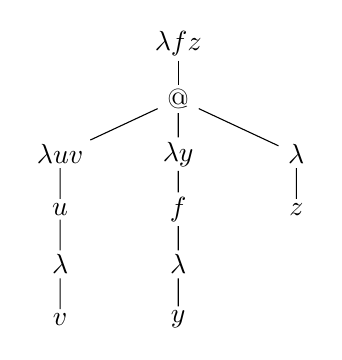
\begin{tikzpicture}[level distance=7mm,inner ysep=0.5mm]
 \node {$\lambda f z$}
    child {
        node {@}
        child {
            node {$\lambda u v$}
            child{
                node{$u$}
                child {
                    node{$\lambda$}
                    child {
                        node{$v$}
                    }
                }
            }
        }
        child {
            node {$\lambda y$}
            child{
                node {$f$}
                child{
                    node {$\lambda$}
                    child { node {$y$} }
                }
            }
        }
        child {
            node {$\lambda$}
            child{ node {$z$} }
            }
        };
\end{tikzpicture}
\end{columns}
}


\frame{
\frametitle{Justified sequence}

\begin{itemize}
\item  We define an \highlight{enabling relation} $\vdash$ on the set of nodes:
\begin{itemize}
  \item a bound variable is enabled by its binder;
  \item a free variable is enabled by the root $\theroot$;
  \item a lambda node  is enabled by its parent node;
  \item an @-node has no enabler.
\end{itemize}

\item Distinction between external nodes $N^{\theroot\vdash}$(hereditarily justified by the root) and the internal nodes $N^{@\vdash}$ (her.\ just.\ by an @-node).

\item A \highlight{justified sequence} is a sequence of nodes such that all the non @-nodes have a justification pointer respecting the relation $\vdash$.

\item  The analogy with game semantics is:
\begin{itemize}
\item $\lambda$-nodes $\equiv$ O-moves
\item @-nodes and variable-nodes $\equiv$ P-moves
\end{itemize}

We can define notions of P-view and O-view, alternation, P-visibility, O-visibility.
\end{itemize}
}




\frame{
\frametitle{Traversals rules}
The computation is described by a set $\travset(M)$ of justified sequences called \highlight{traversals} and given by induction over the rules:
%\begin{FramedTable}
%\noindent {\bf Initialization rules}
\begin{itemize}[]
\item\rulenamet{Empty} $\epsilon \in\travset(M)$
\item \rulenamet{Root} $\theroot \in \travset(M)$
%\end{itemize}
%\noindent {\bf Structural rules}
%\begin{itemize}[]
    \item \rulenamet{Lam} $t \cdot \lambda \overline{\xi} \in\travset(M) \implies t \cdot \lambda \overline{\xi} \cdot n \in\travset(M)$ where $n$
        is $\lambda \overline{\xi}$'s child and is justified by the only occurrence of
        its enabler in the P-view
    \item \rulenamet{App}  $t \cdot @ \in\travset(M) \implies$ \Pstr[0.4cm]{t \cdot (m) @  \cdot (n-m,40:0) n} $\in\travset(M)$.
%\end{itemize}
%\emph{\bf Input-variable rules}
%\begin{itemize}[]
\item \rulenamet{ExtVar} $t\cdot x\in\travset(M)$, $x\in N^{\theroot\vdash}_{\sf var}$ $\implies$
$t \cdot x \cdot n \in\travset(M)$
for any $\lambda$-node $n$ justified by some
occurrence of its parent node in $\oview{t}$.

%\item \rulenamet{ContextValue} If $t_1
%\cdot x \cdot t_2 \in\travset(M)$ with pending node $x \in
%N_{\sf var}^{\theroot\vdash}$ then so is \Pstr[0.5cm]{t_1 \cdot
%(x){x} \cdot t_2 \cdot (xv-x,38:v){v_x} } for all $v \in
%\mathcal{D}$.
%\end{itemize}
%\emph{\bf Copy-cat rules}
%\begin{itemize}[]
\item\rulenamet{IntVar}
\Pstr[0.2cm]{t \cdot (n){n} \cdot (lx){\lambda \overline{x}}
    \ldots (x-lx,40:i){x_i} } $\in\travset(M)$, $x_i \in
    N_{\sf var}^{@\vdash} \implies$  \Pstr[0.5cm]{ t \cdot
(n){n} \cdot (lx){\lambda \overline{x}}  \ldots (x-lx,25:i){x_i}
    \cdot (letai-n,32:i){\lambda \overline{\eta_i}}} $\in\travset(M)$.
%\item\rulenamet{Value}
%  If \Pstr{t \cdot (m){m} \cdot (n){n}  \ldots
%(vn-n,50:v){v}_{n} } $\in\travset(M)$ where $n\in N$ then
%\Pstr[0.6cm]{t \cdot (m){m} \cdot (n){n} \ldots
%(vn-n,50:v){v}_{n} \cdot (vm-m,45:v){v}_m} $\in\travset(M)$.
\end{itemize}
%\caption[Traversal rules for the simply-typed
%lambda-calculus]{Traversal rules for the simply-typed
%$\lambda$-calculus.}
%\label{tab:trav_rules}
%\end{FramedTable}

}


\frame{
\frametitle{Example of traversal}


\begin{center}
%\begin{columns}
%\column{6cm}
%\column{3.5cm}
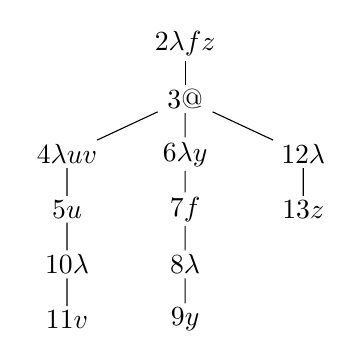
\begin{tikzpicture}[level distance=7mm,inner ysep=0.5mm]
 \node {\highlightat{2}{$\lambda f z$}}
    child {
        node {\highlightat{3}{@}}
        child {
            node {\highlightat{4}{$\lambda u v$}}
            child{
                node{\highlightat{5}{$u$}}
                child {
                    node{\highlightat{10}{$\lambda$}}
                    child {
                        node{\highlightat{11}{$v$}}
                    }
                }
            }
        }
        child {
            node {\highlightat{6}{$\lambda y$}}
            child{
                node {\highlightat{7}{$f$}}
                child{
                    node {\highlightat{8}{$\lambda$}}
                    child { node {\highlightat{9}{$y$}} }
                }
            }
        }
        child {
            node {$\highlightat{12}{\lambda}$}
            child{ node {\highlightat{13}{$z$}} }
            }
        };
\end{tikzpicture}
%\end{columns}
\end{center}

\setbox0=\hbox{$\textcolor{blue}{
\pstr{\only<2->{\nd t= (n0){\lambda f z}}
        \only<3->{\nd\cdot (n1){@}}
        \only<4->{\nd\cdot (n2-n1){\lambda u v}}
        \only<5->{\nd\cdot (n3-n2){u}}
        \only<6->{\nd\cdot (n4-n1){\lambda y}}
        \only<7->{\nd\cdot (n5-n0){f}}
        \only<8->{\nd\cdot (n6-n5){\lambda }}
        \only<9->{\nd\cdot (n7-n4){y}}
        \only<10->{\nd\cdot (n8-n3){\lambda }}
        \only<11->{\nd\cdot (n9-n2){v}}
        \only<12->{\nd\cdot (n10-n1){\lambda }}
        \only<13->{\nd\cdot (n11-n0){z}}
}}$}
\ht0 2cm\box0 % Make sure the height of box containing the traversal remains constant across the different generated slides

}

\frame{
\frametitle{Operations on traversals}
$\pstr{\nd t= (n0){\lambda f z}
        \nd\cdot (n1){@}
        \nd\cdot (n2-n1){\lambda u v}
        \nd\cdot (n3-n2){u}
        \nd\cdot (n4-n1){\lambda y}
        \nd\cdot (n5-n0){f}
        \nd\cdot (n6-n5){\lambda }
        \nd\cdot (n7-n4){y}
        \nd\cdot (n8-n3){\lambda }
        \nd\cdot (n9-n2){v}
        \nd\cdot (n10-n1){\lambda }
        \nd\cdot (n11-n0){z}
}$
\vspace*{0.4cm}
\begin{itemize}
\item The \highlight{reduction of a traversal} is obtained by keeping only
the occurrences hereditarily justified by the root:
$$\color{red}{ \Pstr[0.7cm]{t \filter \lambda f z = (n0){\lambda f z}\ (n1-n0){f}\ (n2-n1){\lambda }\ (n3-n0){z} } }$$
\pause

\item  \highlight{\it @-nodes removal:}
$$\Pstr[0.5cm]{ t - @ = (n0){\lambda f z}\ (n1-n0){\lambda u v}\ (n2-n1){u}\ (n3-n0){\lambda y}\ (n4-n0){f}\ (n5-n4){\lambda }\ (n6-n3){y}\ (n7-n2){\lambda }\ (n8-n1){v}\ (n9-n0){\lambda }\ (n10-n0){z}}$$
\end{itemize}

}


\subsection{The Correspondence Theorem}
\frame{ \frametitle{The Correspondence Theorem}
\begin{block}{}
Let $M$ be a simply typed term of type $T$. There exists a function $\textcolor{DarkGreen}{\varphi}$
from the nodes of the \highlight{computation tree} to the
moves of the \highlight{arenas} of $\revsem{T}$ such that
$$ \textcolor{DarkGreen}{\varphi}  : \travset(M)^{-@} \textcolor{DarkGreen}{\stackrel{\cong}{\longrightarrow}}
\revsem{M} $$
$$ \textcolor{DarkGreen}{\varphi}  : \travset(M)^{\filter \theroot}  \textcolor{DarkGreen}{\stackrel{\cong}{\longrightarrow}} \sem{M} \ .$$
\end{block}
where
\begin{itemize}
\item $\highlight{\travset(M)}$ = set of traversals of the computation tree of $M$
\item $\highlight{\travset(M)^{\filter \theroot}} = \{ t \filter t_0 \ | \  t\in\travset(M) \}$
\item $\highlight{\travset(M)^{-@}} = \{ t - @ \ | \  t \in {\travset(M)} \}$
\item $\highlight{\sem{M}}$ = game-semantic denotation of $M$
\item $\highlight{
\revsem{M}}$ = revealed denotation of $M$.
\end{itemize}

}


\frame{ \frametitle{More correspondences}
\begin{center}
\begin{tabular}{c|c}
Computation tree notions & Game-semantic equivalents \\ \hline \hline \\
computation tree & arena(s) \\ \\
traversal & uncovered play \\ \\
reduced traversal & play \\ \\
path in the computation tree & P-view of an uncovered play
\end{tabular}
\end{center}
\note{Innocence $\leftrightarrow$ the next node to visit after a $\lambda$-node is determined by the current position in the syntax tree.}
}


\subsection{Example}
\frame{\frametitle{Example:
 $\vdash \lambda f^{o \typear o} .
(\lambda u^{o \typear o} . u) f : (o \typear o) \typear
o \typear o$}

Left: computation tree. Right: arena.
\begin{center}
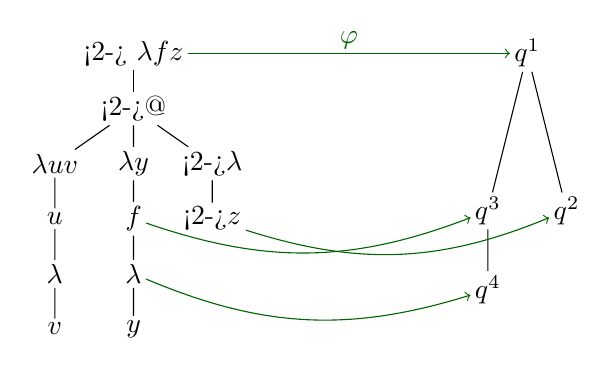
\begin{tikzpicture}[level distance=7mm,inner ysep=0.5mm,inner xsep=0.5mm,sibling distance=10mm]
%\color{blue}
\node (root) {\only<2->{\color{red}}
$\lambda f z$}
    child{
      node{\only<2->{\color{red}}$@$}
          child{
            node {$\lambda u v$}
            child{
              node (u) {$u$}
              child{
                node (lmd) {$\lambda$}
                child{
                  node {$v$}
                }
              }
            }
          }
          child{
            node {$\lambda y$}
            child{
                node (h) {$f$}
                child{
                  node (h1) {$\lambda$}
                  child{
                    node {$y$}
                  }
                }
            }
          }
          child{
            node {\only<2->{\color{red}}$\lambda$}
            child{
              node (z) {\only<2->{\color{red}}$z$}
            }
          }
      }
;
%\color{red}
\draw +(5,0) node (q1) {$q^1$}
    [level distance=20mm]
%      child{
%        node (q5) {$q^5$}
%        [level distance=10mm]
%        child{ node (q6) {$q^6$} }
%      }
      child{
        node (q3) {$q^3$}
        [level distance=10mm]
        child{ node (q4) {$q^4$} }
      }
      child{ node (q2) {$q^2$} }
;
\color{DarkGreen}
\draw[->] (root) -- node[above] {$\varphi$} (q1);
\draw[->] (h) to [bend right=20]  (q3);
\draw[->] (h1) to [bend right=20]  (q4);
\draw[->] (z) to [bend right=20]  (q2);
\end{tikzpicture}
\end{center}
\begin{itemize}
\item $\pstr{\nd t= (n0){\lambda f z}
        \nd\cdot (n1){@}
        \nd\cdot (n2-n1,35){\lambda u v}
        \nd\cdot (n3-n2,35){u}
        \nd\cdot (n4-n1,35){\lambda y}
        \nd\cdot (n5-n0,35){f}
        \nd\cdot (n6-n5,35){\lambda }
        \nd\cdot (n7-n4,35){y}
        \nd\cdot (n8-n3,35){\lambda }
        \nd\cdot (n9-n2,35){v}
        \nd\cdot (n10-n1,35){\lambda }
        \nd\cdot (n11-n0,35){z}
}$

\pause
\item $\Pstr{\color{red}\pview{t} = (q1){\color{red}\lambda f z} \cdot (n2){\color{red}@}
\cdot (n9-n2,35){\color{red}\lambda}
\cdot (q2-q1,35){\color{red}z}}$
\pause

\item
$
\textcolor{DarkGreen}{
\varphi (} %\textcolor{blue}
{t \filter \lambda f z}
\textcolor{DarkGreen}{)} = \textcolor{DarkGreen}{\varphi (}
\textcolor{blue}{
\Pstr[70mm]{ (q1){\lambda f z}
            \cdot (q3-q1){f}
            \cdot (q4-q3){\lambda}
            \cdot (q2-q1){z} }
}
\textcolor{DarkGreen}{)} = %\textcolor{red}
{
\Pstr[70mm]{
    (q1){q}^1\
    (q5-q1){q}^3\
    (q6-q3){q}^4\
    (q2-q1){q}^2
}}
\in %\textcolor{red}
{\sem{M}}.
$

\end{itemize}
}



\begingroup
\newcommand\sigcol[1]{{\color{blue} #1}}
\newcommand\mucol[1]{{\color{red} #1}}
\newcommand\mynodeex[3]{\node[name=#2]{\only<#1->{$#3$}};}


\subsection{Composition}
\begin{frame}[fragile]
\frametitle{Composition}

$$\sem{M};\sem{N} = \sem{\lambda x . N (M x)}$$
\pause
Example:
\begin{itemize}
\item $A=o$, $B=o\typear o$, $C=((o\typear o)\typear o)\typear o$
\item
$\sigcol{\sigma} = \sem{ \sigcol{\lambda x^o v^o .x} : A\typear B}$
\item $\mucol{\mu} = \sem{ \mucol{\lambda y^B \varphi^{((o\typear o)\typear o)}. \varphi (\lambda u^o.y(\lambda.u))} : B \typear C}$
\end{itemize}

We then have $\sigcol{\sigma} \fatcompos \mucol{\mu} = \sem{ \lambda x \varphi. \varphi (\lambda u . x) : A \typear C}$.
\bigskip

\begin{tikzpicture}
  [style={anchor=base}]
  \matrix[matrix of nodes]
  {
    o & $\stackrel{\sigcol{\sigma}}\longrightarrow$ & ($o\typear$ & o) & $\stackrel{\mucol{\mu}}\longrightarrow$ &  ((($o\typear$ &o)$\typear$ & o)$\typear$ & o) \\
&&&&&&& &  \mynodeex{2}{n0}{\lambda x \varphi \omove  \mucol {\lambda y \varphi}}\\
&&&&&&&\mynodeex{3}{n1}{\varphi  \pmove \mucol \varphi}\\
&&&&&&\mynodeex{4}{n2}{\lambda u \omove  \mucol {\lambda u}} \\
&&&  \mynodeex{5}{n3}{\sigcol {\lambda x v} \opmove \mucol y} \\
\mynodeex{6}{n4}{x \pmove \sigcol x}\\
  };
\only<3->{\draw[->] (n1) .. controls +(60:0.2cm) and +(-0.4cm,0) .. (n0.west);}
\only<4->{\draw[->] (n2) .. controls +(60:0.2cm) and +(-0.4cm,0) .. (n1.west);}
\only<5->{\draw[->] (n3) .. controls +(30:1cm) and +(-1,0) .. (n0.west);}
\only<6->{\draw[->] (n4) .. controls +(30:1cm) and +(-1,0) .. (n3.west);}
\only<6->{\draw[->] (n4) .. controls +(60:1cm) and +(-1,0) .. (n0.west);}
\end{tikzpicture}
\end{frame}
\endgroup


\subsection{Demo}
\frame{\frametitle{Tool demo}
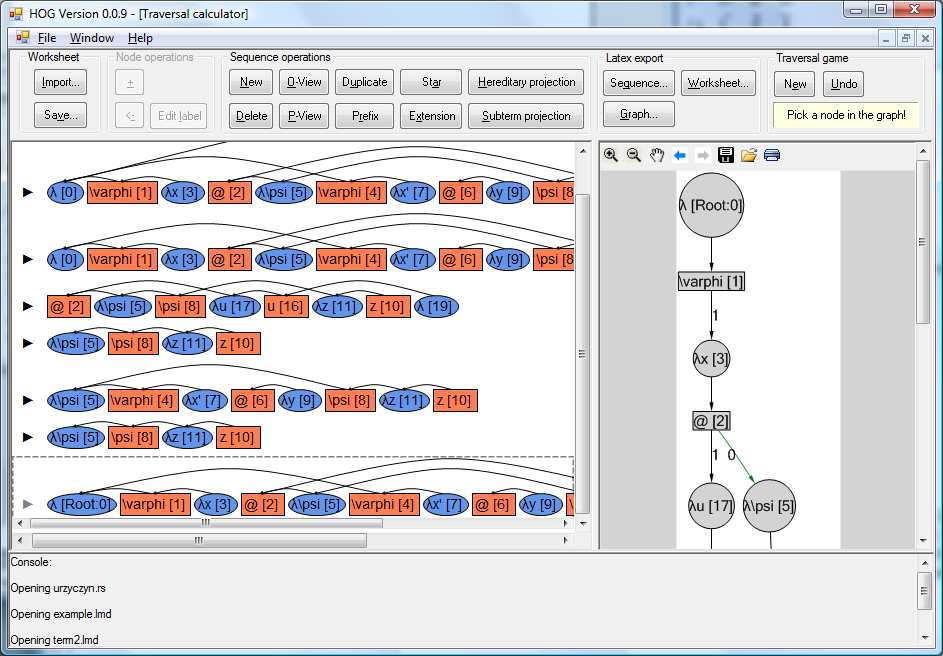
\includegraphics[width=11cm]{sshot.jpg}

}

\frame{\frametitle{Benefits}

\begin{itemize}
  \item \highlight{Pedagogical:} Game semantics is sometimes considered hard to understand. Partly because of some obscure technical definitions.
      \begin{itemize}
        \item A \highlight{P-view} is just a \highlight{control point} in the program AST. The \highlight{O-view} is the dual \ie the control point of the environment;

        \item \highlight{Innocence} means that the current control point determines the next action taken by the program.

        \item Adding reference variables breaks innocence because of side-effects.
          
        \item \highlight{Visibility} restricts the program to access only code that is in scope.

        \item Adding general reference breaks visibility: \eg\ $\ianew\ {\tt x} := \lambda y .y {\tt\ in\ } x~a;$
                          
      \end{itemize}
  
  \item \highlight{Efficient:} top-down computation of the game denotation as opposed to a compositional bottom-up approach.
      \begin{itemize}
        \item only the relevant O-moves of the subterms are considered;
        \item hiding performed only once at the end;
        \item composition can be done at the syntactic level;
        \item traversals ending with an internal move have an O-view
        of length $\mathcal{O}(\ord{M})$.
      \end{itemize}
      
  
  
\end{itemize}
}




%%%%%%%%%%%%%%%%%%%%%%%%%%%%%%%%%%%%%%%%%%%%%%%%%

\section{Applications}


\subsection{Higher-order grammars}
\frame{\frametitle{Higher-order grammars}
%\emph{Notation for types:} $A_1 \rightarrow (A_2 \rightarrow (\ldots (A_n \rightarrow o)) \ldots )$
%is written $(A_1,A_2,\ldots, A_n,o)$.

\begin{itemize}
\item A \highlight{higher-order grammar} is formally given by a tuple
$\langle \Sigma, \mathcal{N}, \mathcal{R}, \mathcal{S} \rangle$
(terminals, non-terminals, rewritting rules, starting symbol)

\item Higher-order grammars used as generators of word languages or trees are called \highlight{recursion schemes} (Maslov, 1974).

\item Example of a tree-generating order-2 recursion scheme:
\begin{columns}
      \column{.3\textwidth}
$\begin{array}{rll}
  S & \rightarrow & H \, a\\
  H \, z^o & \rightarrow & F \, (g \,
  z)\\
  F \, \phi^{o\typear o} & \rightarrow & \phi \, (\phi \, (F \, h))\\
\end{array}$
      \column{.3\textwidth}
\begin{tikzpicture}[baseline=(root.base),level distance=5mm,inner ysep=0.5mm,sibling distance=10mm]
 \node (root) {$g$}
    child {node {$a$}}
    child {node {$g$}
        child { node{$a$} }
        child { node{$h$}
                child { node{$h$}
                        child { node{$\vdots$} }
                }
        }
    } ;
\end{tikzpicture}
\end{columns}
Terminals: $a:o$ and $g,h:o\typear o$. Non-terminals: $S :o$, $H:o\typear o$ and $F:(o\typear o)\typear o $.
\end{itemize}
}

\frame{
\frametitle{Tree generating Higher-Order Pushdown Automata}
HOPDAs generalize PDAs to nested stacks: a 1-PDA is a standard PDA; an order $n$-HOPDA manipulates a stack with $n$ levels of nesting.

Formally given by a tuple $\langle Q,\Sigma,\Gamma,\delta,q_o,\bot\rangle$
where $\delta \subseteq Q\times \Gamma \rightarrow Q \times {\sf Op}_n$
and the operations of ${\sf Op}_n$ are:
\begin{itemize}
    \item $push_1 a$: pushes the element $a$ on the top level $1$-stack;
    \item $pop_1$: pops the top element of the top level $1$-stack;
    \item $push_j$, $j>1$: duplicates the top level $j-1$-stack;
    \item $pop_j$, $j>1$: deletes the top level $j-1$-stack.
\end{itemize}
Additionally, we have an operation for generating tree-node:
\begin{itemize}
  \item $emit_f (q_1, \ldots, q_k)$, for each node-constructor $f:o^k\typear o \in \Sigma$.
\end{itemize}

\begin{theorem}
For generating word or tree languages, order-$n$ pushdown automata
are equivalent to order-$n$ \highlight{safe} recursion scheme [Damm82,KNU02].
\end{theorem}
What is the automata equivalent of unrestricted recursion schemes?
}

\frame{
\frametitle{Collapsible Pushdown Automaton (CPDA)}
\begin{itemize}
\item Hague, Murawski, Ong, Serre, LICS08:
\begin{itemize}
    \item it is an extension of HOPDA where each symbol in the stack can have a pointer to a sub-stack occurring underneath it;
    \item it can ``collapse'' the stack by following the pointer associated to the top element.
\end{itemize}

\item There is a transformation from HORS to CPDA and conversely.

\item The first transformation is based on the traversal theory:
\begin{enumerate}[1.]
  \item compute the computation graph of the HORS by taking the $\eta$-long nf of each grammar rule;
  \item construct a CPDA ``simulating'' the HORS by calculating the traversals of its computation graph. This is possible because the computed term is of ground type.
\end{enumerate}
\pause
\item Tool demo...
\end{itemize}

}

\subsection{Other applications}
\frame{\frametitle{Other applications, related works}

\begin{itemize}
\item \highlight{Verification:}  Knapik {\it et.\ al.} (2002) showed that \highlight{MSO model checking} for trees generated by HORS
 of any order and verifying the \highlight{safety restriction} (a syntactic restriction that constrains the occurrences of variables according to their orders) is decidable.

    Using the notions of computation tree/traversal Ong was able to show (LICS06) that this result still holds in the unrestricted case.
%\item Ong introduced computation trees in LICS2006 to prove decidability of MSO theory on infinite trees
%generated by higher-order grammars.

\pause

\item Studying the effect of syntactic restrictions on the game semantics model.
 \eg\ One can show that \highlight{pointers are uniquely recoverable} in the game denotation of terms satisfying the safety restriction.
\pause

\end{itemize}

\highlight{Related works:}

\begin{itemize}
\item Stirling recently proved decidability of higher-order pattern matching with a game-semantic approach
 relying on equivalent notions of computation tree and traversal.
\end{itemize}
}



%%%%%%%%%%%%%%%%%%%%%%%%%%%%%%%%%%%%%%%%%%%%%%%%%
%\subsection{Simply Typed \texorpdfstring{$\lambda$}{Lambda}-Calculus}
%\frame{\frametitle{Simply Typed $\lambda$-Calculus}
%\begin{itemize}
%\item \highlight{Simple types} $A := o\ |\ A \rightarrow A$.
%%We write $(A_1,\ldots, A_n)$ for $A_1\rightarrow \ldots \rightarrow A_n$.
%
%\item The \highlight{order} of a type is given by $\textsf{order}(o) = 0$,
%$\textsf{order}(A \rightarrow B) = \max(\textsf{order}(A) + 1, \textsf{order}(B))$.
%
%
%\end{itemize}
%}
%



\section{Conclusion \& Future Works}
\frame{ \frametitle{Conclusion \& Future Works}

\begin{itemize}
\item \highlight{Conclusion:} a new \highlight{concrete} way to present game semantics
based on the theory of \highlight{traversals}.

\item \highlight{Future works:} \hfill

\begin{itemize}
\item Extend the correspondence to PCF and Idealized Algol;
\item Can we generalize CPDA to give an automata characterization of the simply-typed lambda calculus?
\item Consider the Reachability problem in the traversal setting,
\item Complexity: characterization of space-complexity classes by analyzing the length of the traversals? (See Kazushige Terui's work.);
\item Implement other transformations: from CPDA to HORS and from safe HORS to PDA;
\item Implement the MSO decision procedure.
\end{itemize}

\end{itemize}
}

\begin{frame} \frametitle<presentation>{Bibliography}

  \begin{thebibliography}{10}
  \beamertemplatearticlebibitems
    \bibitem{abramsky:game-semantics-tutorial}
    S.~Abramsky and G.~McCusker
    \newblock Game semantics, Lecture notes.
    \newblock In {\em Proceedings of the 1997 Marktoberdorf Summer School}. 1998.

    \bibitem{localbeta2008}
    W.~Blum and C.-H.~L.~Ong
    \newblock Local computation of beta-reduction
    \newblock Technical report. University of Oxford, 2008.

%    \bibitem{safety-mirlong2004}
%    Klaus Aehlig, Jolie~G. de~Miranda, and C.-H.~Luke Ong.
%    \newblock Safety is not a restriction at level 2 for string languages.
%    \newblock Technical report. University of Oxford, 2004.

    \bibitem{hague-sto07}
    M.~Hague, A.S.~Murawski, C.-H.~L. Ong and O.~Serre
    \newblock Collapsible pushdown automata and recursive schemes.
    \newblock To appear, LICS2008.

    \bibitem{OngLics2006}
    C.-H.~Luke Ong
    \newblock On model-checking trees generated by higher-order recursion schemes.
    \newblock In {\em Proceedings of LICS2006.}

    \bibitem{DBLP:conf/icalp/Stirling06}
    C.~Stirling
    \newblock A game-theoretic approach to deciding higher-order matching.
    \newblock In {\em Proceedings of ICALP2006.}

  \end{thebibliography}
\end{frame}




\note{
\begin{itemize}
\item nPDA = finite state machines + order n stack
\item For words: 1PDA recognizes context-free language.
        and 0PDA = recognizes regular language.
\item MSO is very expressive: more than the modal mu-calculus (into which LTL CTL CTL* can be embedded.
But over trees, MSO and modal mu-calculus are equi-expressive.)
\item [Caucal02] Graphs generated by safe grammars have a decidable MSO theory.
\item [HMOS06] Caucal's result does not extend to unsafe grammars.
However deciding $\mu$-calculus theories is $n$-EXPTIME complete.
\end{itemize}
}


\end{document}
